\documentclass[a4paper,12pt]{report}            % [forma A4, taille police] {Type}
    \usepackage[utf8]{inputenc}                
    \usepackage[T1]{fontenc}                        % Codage des fontes TeX
    \usepackage[francais]{babel}
    \usepackage{graphicx}
    \usepackage{wrapfig}
    \usepackage{fancyhdr}
    \usepackage{xcolor}
    \usepackage{hyperref}
    \usepackage{listings}
    \usepackage{fullpage}
    \usepackage{eso-pic}
    \usepackage{titlesec}
    \titleformat{\chapter}[hang]{\bf\huge}{\thechapter}{2pc}{}
    \lstset {numbers=left ,stepnumber=1,firstnumber=0,numberfirstline=true}
    \hypersetup{
        bookmarks=true,         % show bookmarks bar?
        unicode=false,          % non-Latin characters in Acrobat’s bookmarks
        pdftoolbar=true,        % show Acrobat’s toolbar?
        pdfmenubar=true,        % show Acrobat’s menu?
        pdffitwindow=false,     % window fit to page when opened
        pdfstartview={FitH},    % fits the width of the page to the window
        pdftitle={My title},    % title
        pdfauthor={Author},     % author
        pdfsubject={Subject},   % subject of the document
        pdfcreator={Creator},   % creator of the document
        pdfproducer={Producer}, % producer of the document
        pdfkeywords={keyword1, key2, key3}, % list of keywords
        pdfnewwindow=true,      % links in new PDF window
        colorlinks=true,       % false: boxed links; true: colored links
        linkcolor=black,          % color of internal links (change box color with linkbordercolor)
        citecolor=green,        % color of links to bibliography
        filecolor=magenta,      % color of file links
        urlcolor=blue           % color of external links
    }
    
    \author{Samuel HUET \& Thomas COUTANT}
    \title{\huge{\textbf{Analyseur de Réseaux}}}
    
    \begin{document}
\maketitle
\renewcommand{\contentsname}{SOMMAIRE} % Dans le corps du document,avant la commande \tableofcontents.
\tableofcontents

\chapter{Calibrations}
\addcontentsline{toc}{chapter}{Calibrations}

Afin de mesurer avec précision les paramètres S de notre système, il est nécéssaire de
calibrer l'appareil afin de minimiser au possible les erreurs internes. Mais avant l'étape
de la calibration, nous pouvons déjà brancher le système et regarder sur quelle gamme de
fréquence et sur quelle puissance faut il calibrer. 

\begin{center}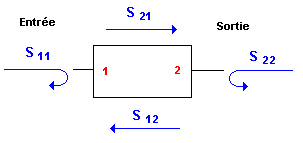
\includegraphics[scale = 0.8]{pic/S.png}\\ \end{center}

Une fois cela fait, nous pouvont aller
dans le menu de calibration en appuyant sur \textbf{CAL}, et voici ce que l'on y trouve :

\begin{center}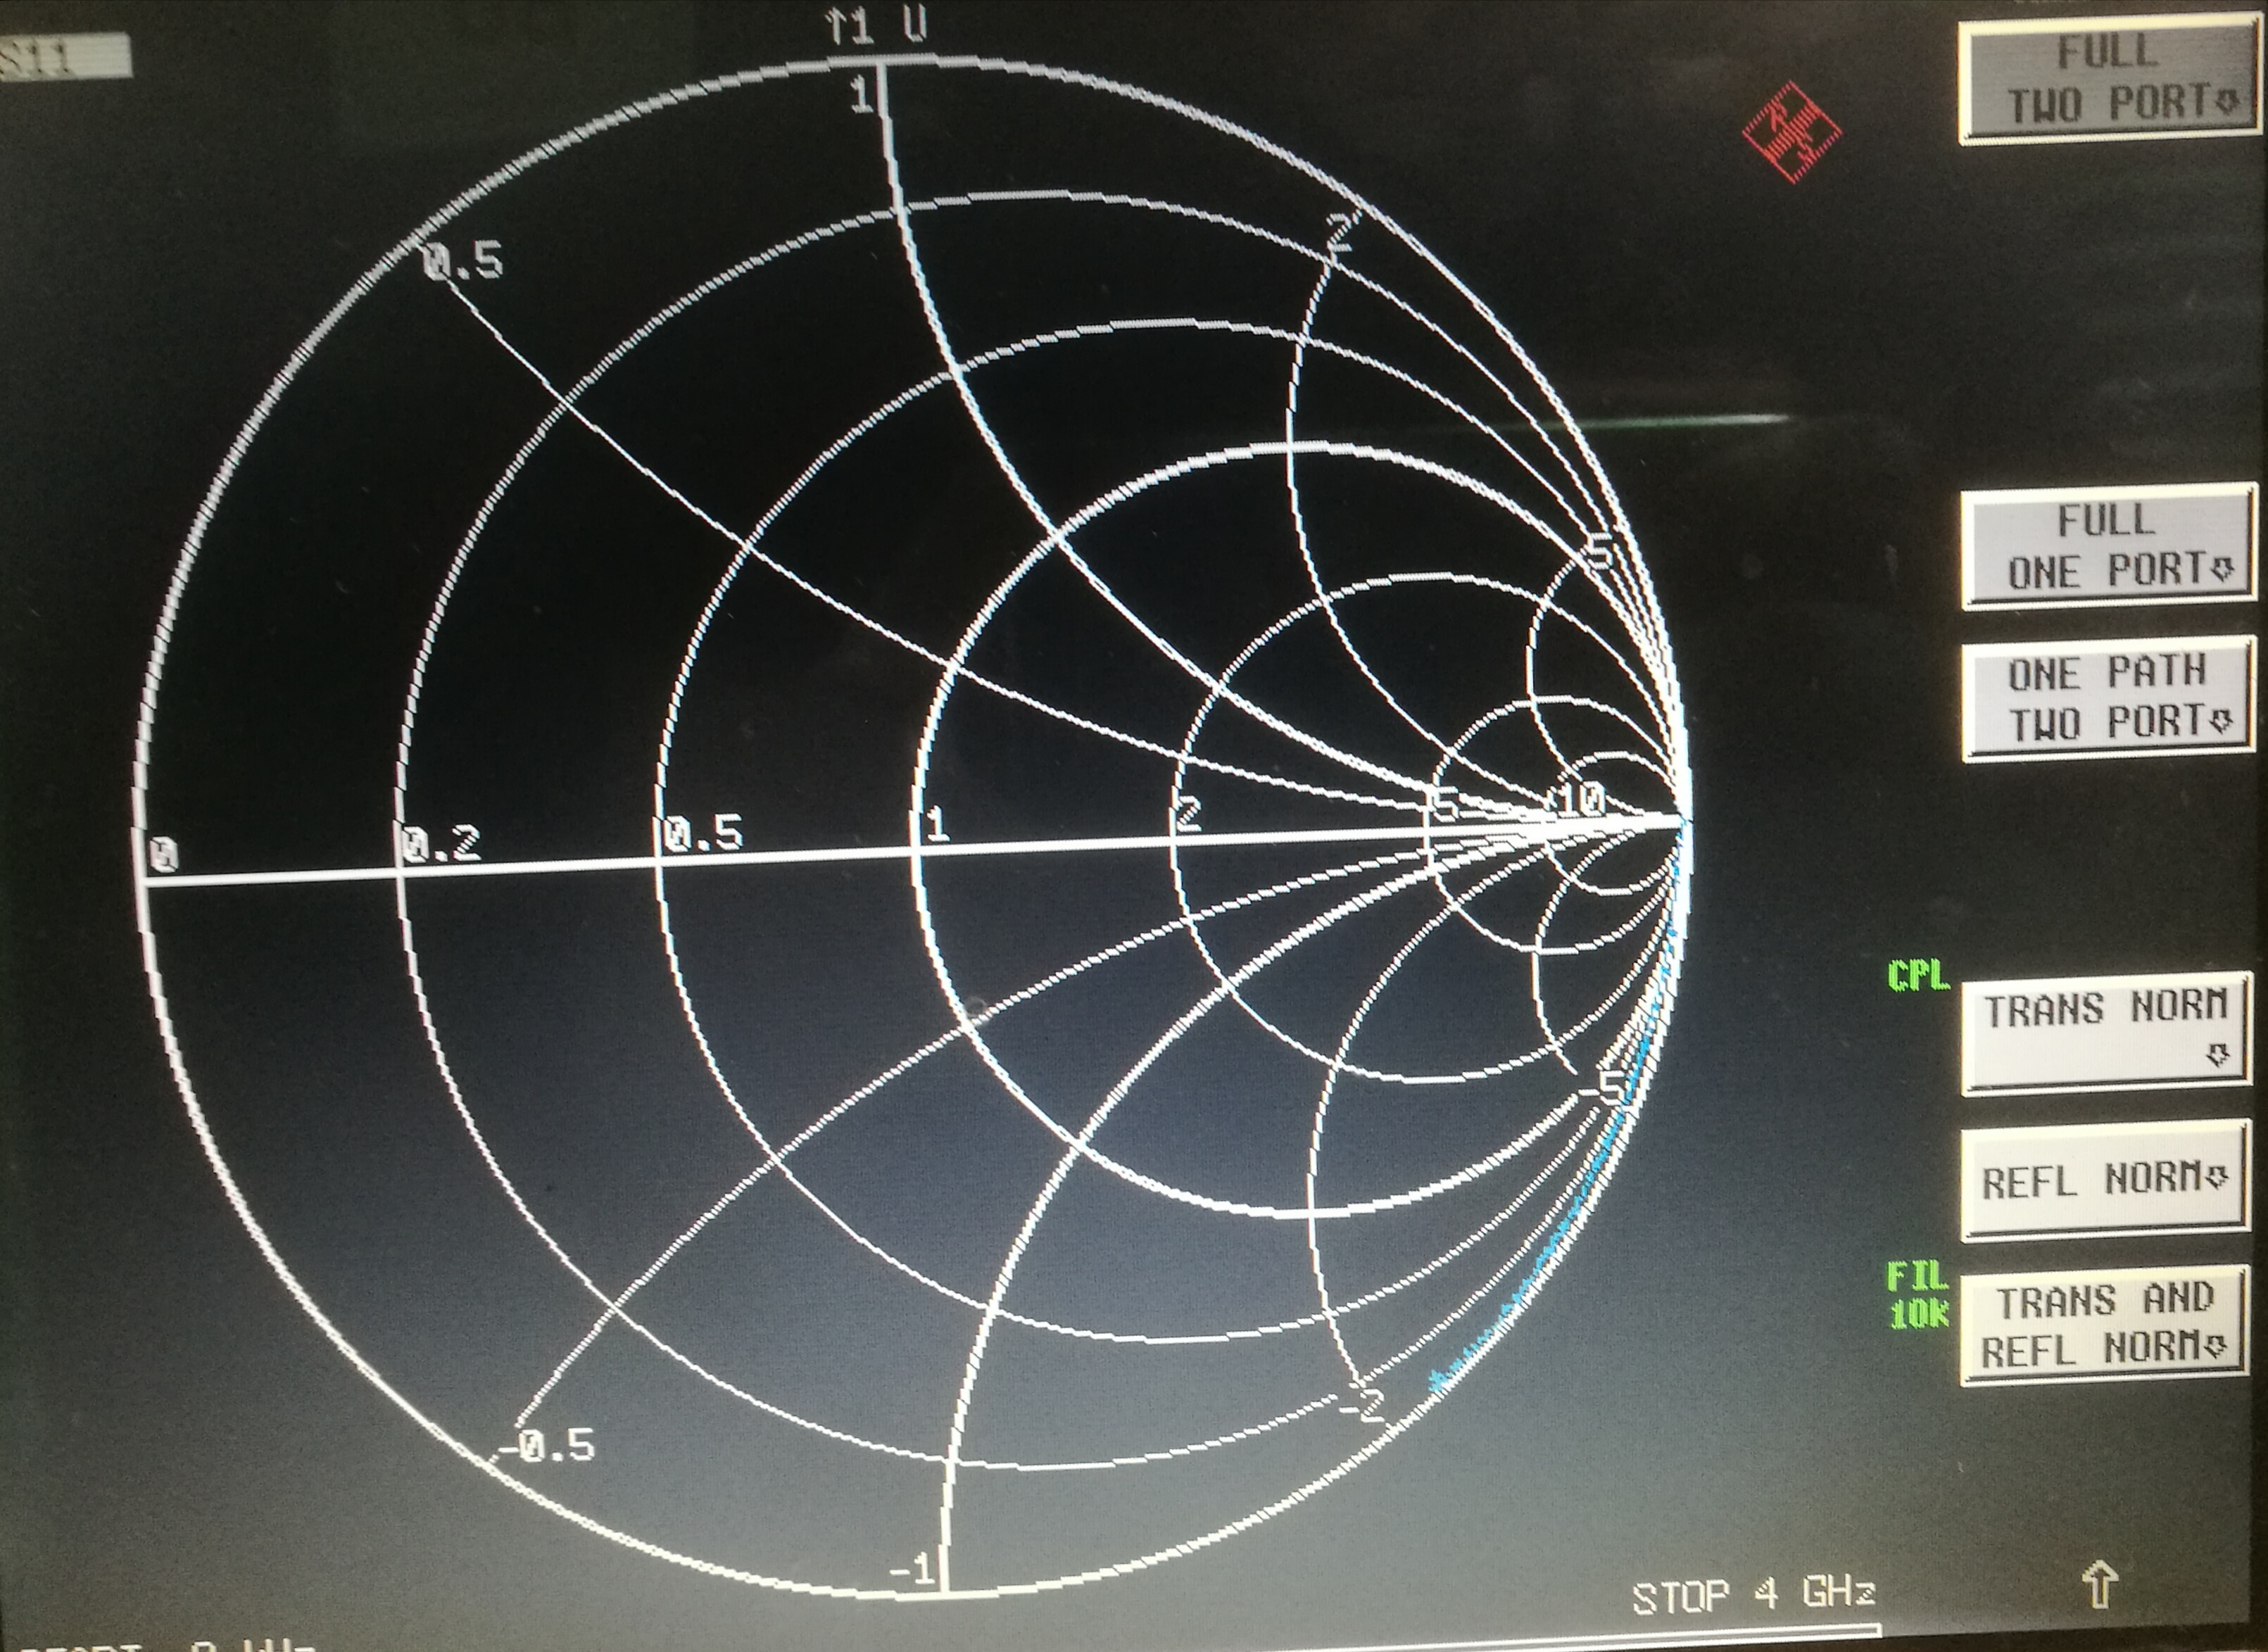
\includegraphics[scale = 0.12]{pic/Calib.jpg}\\ \end{center}

\newpage

\section{Calibrations possibles}
Nous pouvons voir 6 boutons qui correspondent en réalité à 6 types de calibration
différentes :
\begin{itemize}
	\item \textbf{FULL TWO PORT} représente une calibration sur les deux ports, donc des 4 paramètres.
	      C'est la calibration la plus longue car elle nécéssite de brancher et débrancher sur les deux ports.
	\item \textbf{FULL ONE PORT} ne va calibrer uniquement qu'un seul port, afin de calculer les paramètres
	      S11 et S21 (ou S22 et S12)
	\item \textbf{ONE PATH TWO PORT} Ne calibrera que dans le but de mesurer les paramètres S21 et S12.
	\item \textbf{TRANS NORM} ???????
	\item \textbf{REFL NORM} ???????
	\item \textbf{TRANS AND REFL NORM} ???????
\end{itemize}
Pour nos mesures, nous avons utilisé la calibration \textbf{FULL TWO PORT} afin
d'analyser le plus de paramètres possible.  

\section{Connecteur}

Avant de se lancer dans une quelconque manipulation, faisons un petit tour des connecteurs
courants. Dans l'ordre d'apparition, de gauche à droite, nous avons :
\begin{itemize}
	\item Le connecteur \textbf{N}. C'est sur celui-ci que débouchent les ports 1 et 2 de l'analyseur
	\item Le connecteur \textbf{BNC}. Facilement repérable de par sa connecteur en bayonette.
	\item Le connecteur \textbf{SMA}. Plutot petit, il s'addapte bien aux modules (coupleur, mixer, etc). Son
	      composant isolant est en téflon.
	\item Le connectuer \textbf{K}. Ce connecteur est très comparable au SMA, à la seule différence près
	      que sa matière isolante est l'air.
\end{itemize}

\begin{center}
	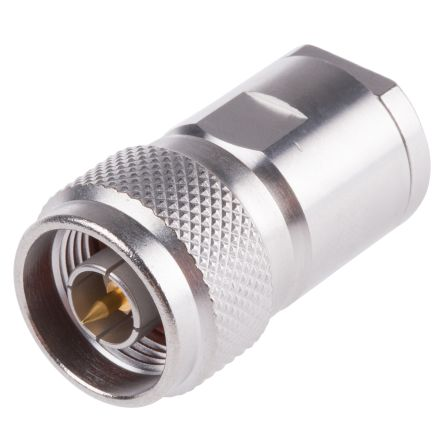
\includegraphics[scale = 0.9]{pic/N.jpg}
	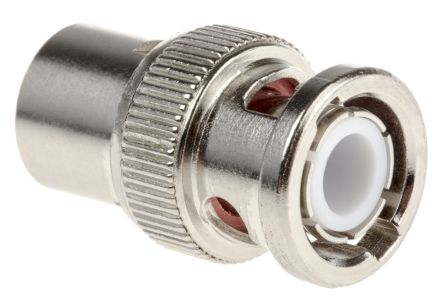
\includegraphics[scale = 0.9]{pic/BNC.jpg}
	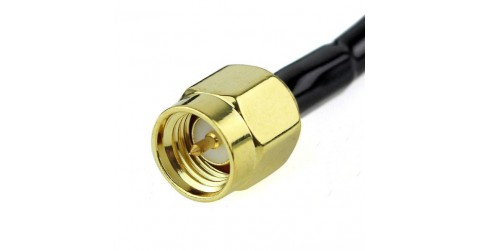
\includegraphics[scale = 0.4]{pic/SMA.jpg}
\end{center}

\chapter{Mesures des filtres}
\addcontentsline{toc}{chapter}{Mesures des filtres}

\section{Cablage}

\begin{center}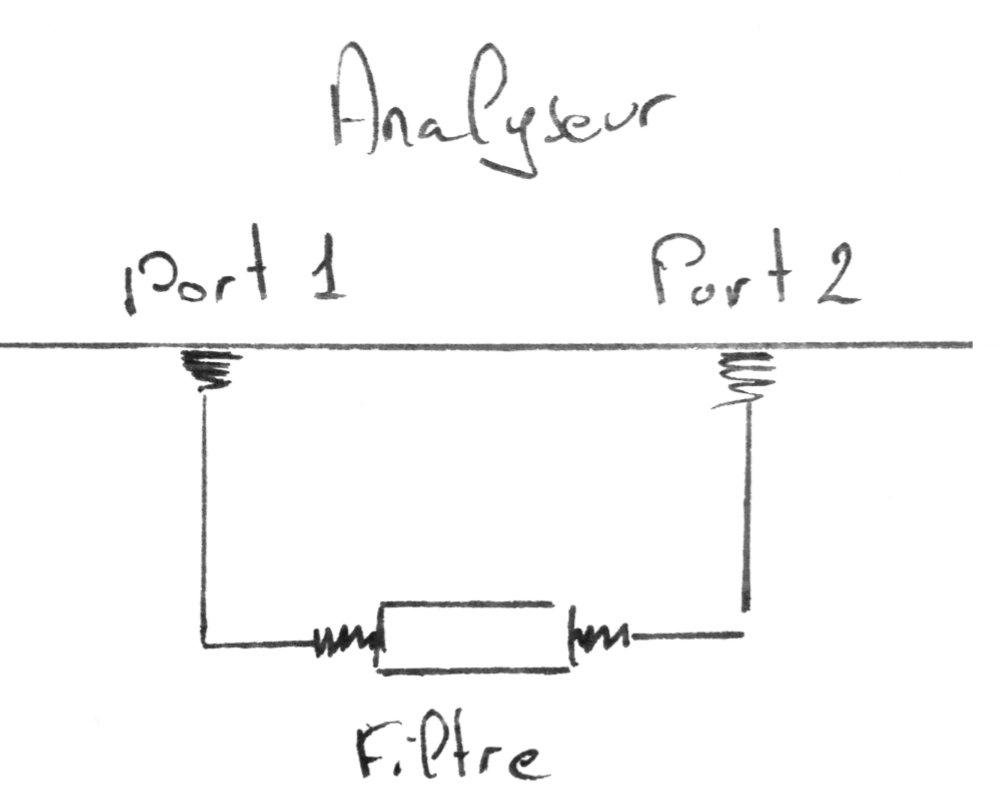
\includegraphics[scale = 0.2]{pic/Cablage_filtre.png}\\ \end{center}

\section{Passe bas}

\begin{center}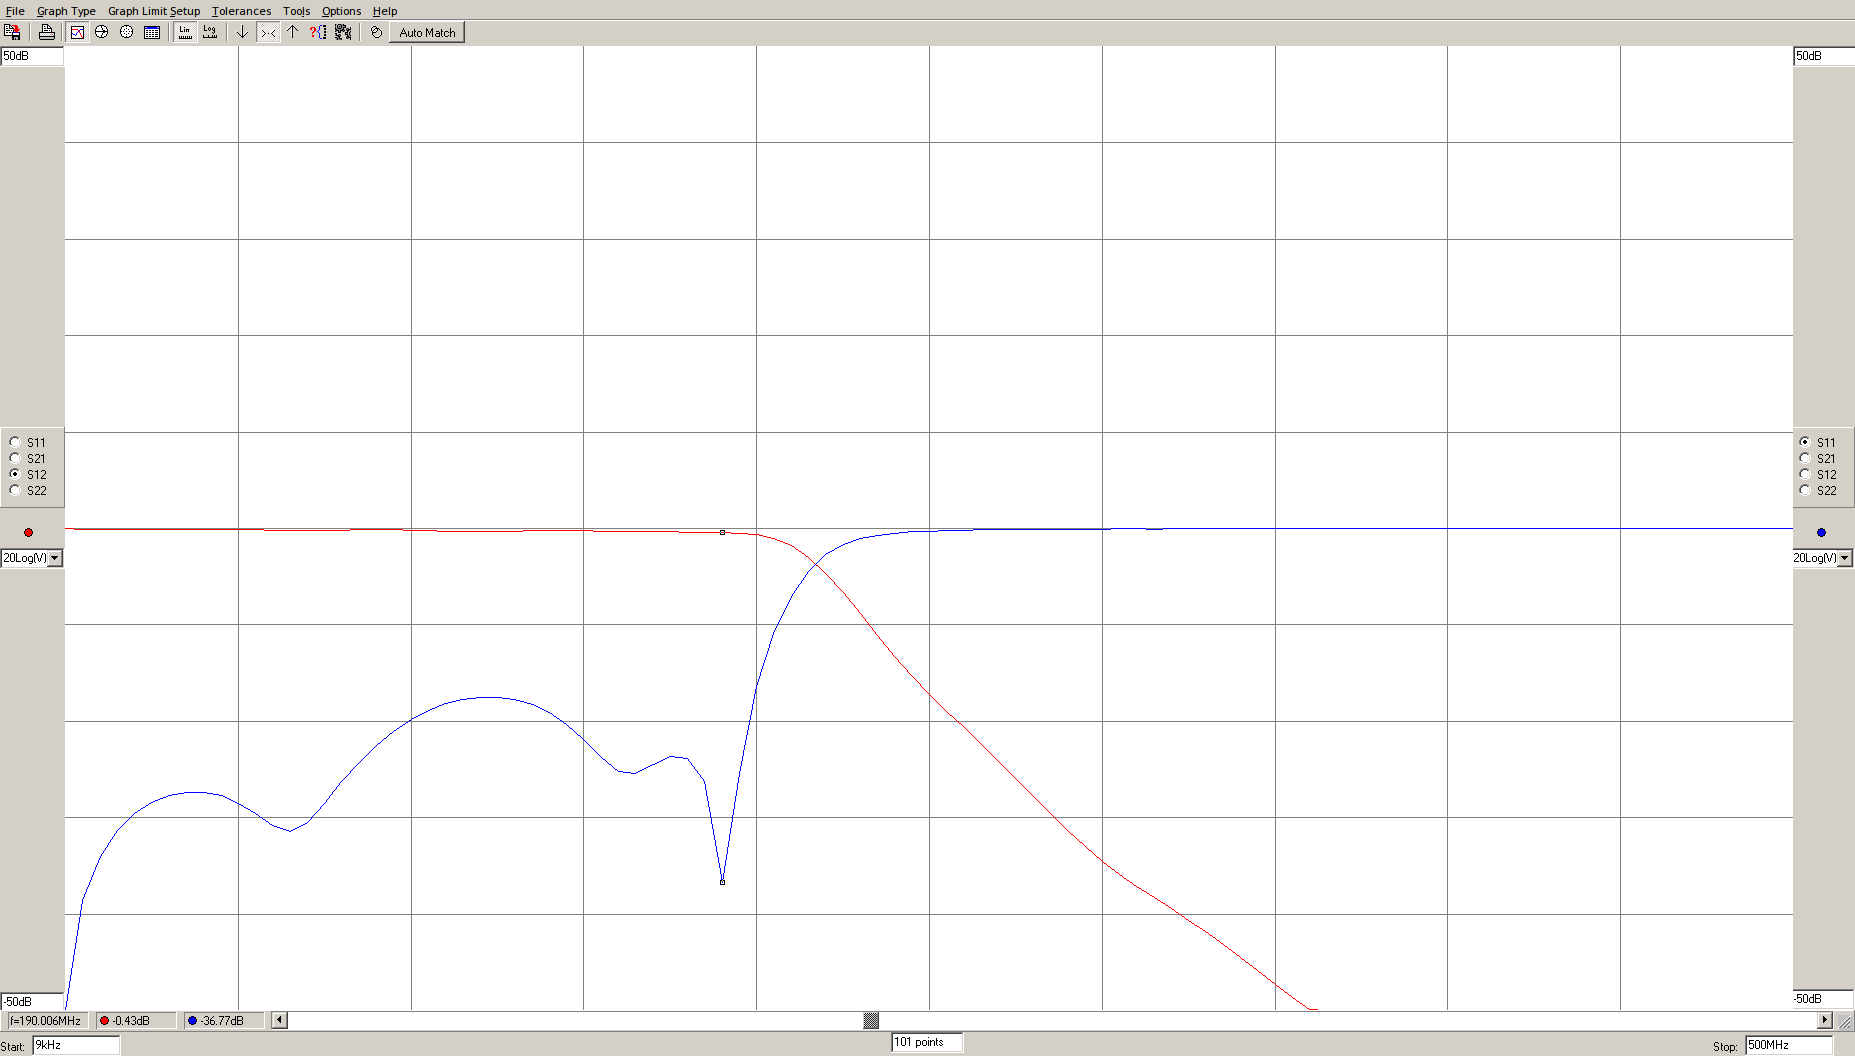
\includegraphics[scale = 0.25]{pic/parametre_passe_bas.png}\\ \end{center}
En rouge nous avons la transmission (S12) et en bleu l'adaptation(S11). On remarque donc facilement que nous avons
à faire à un filtre passe bas. Grâce au logiciele rfsim99 on peut se déplacér librement sur les courbes.
on obtiens donc une fréquence de coupure inferieure à -1dB de 203.747MHz
\begin{center}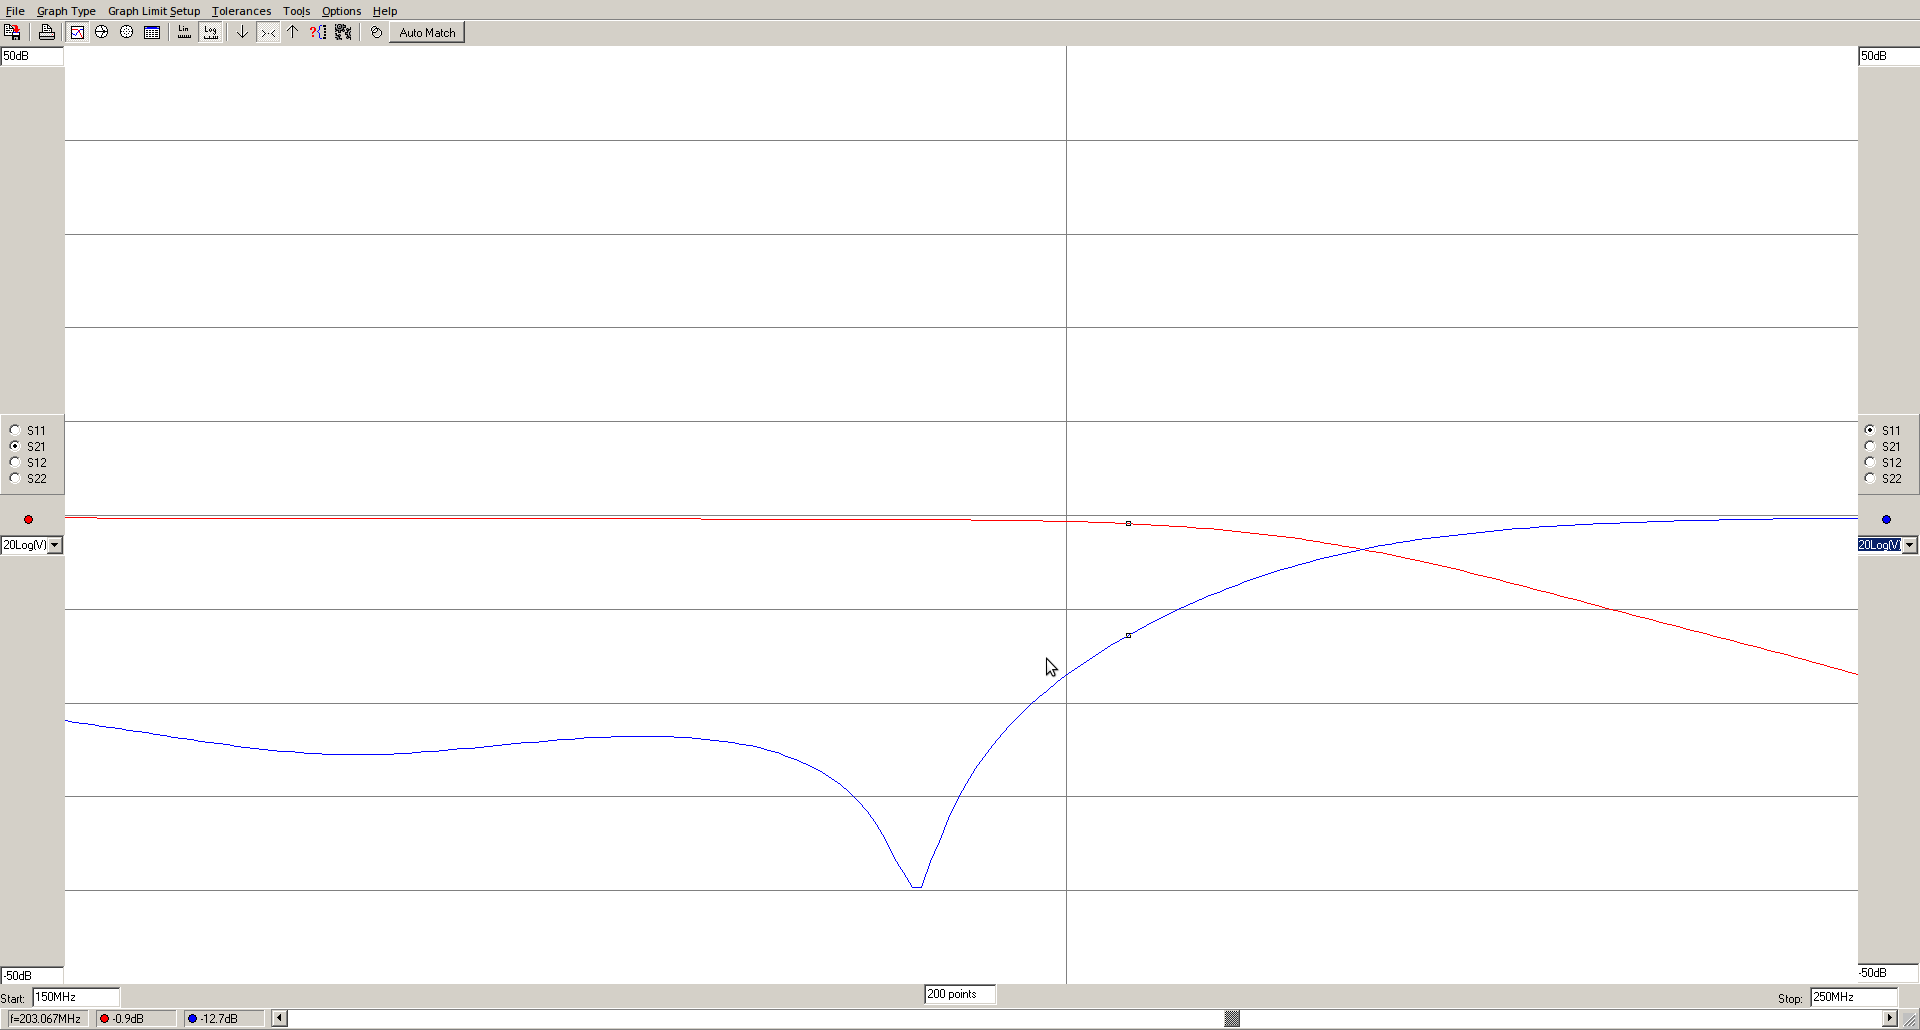
\includegraphics[scale = 0.25]{pic/freq_coupure_pb.png}\\ \end{center}
Les paramètres de réflexions (S11 et S22) sont proche l'un de lautre comme on peut le voir sur le
graphique si dessous
\begin{center}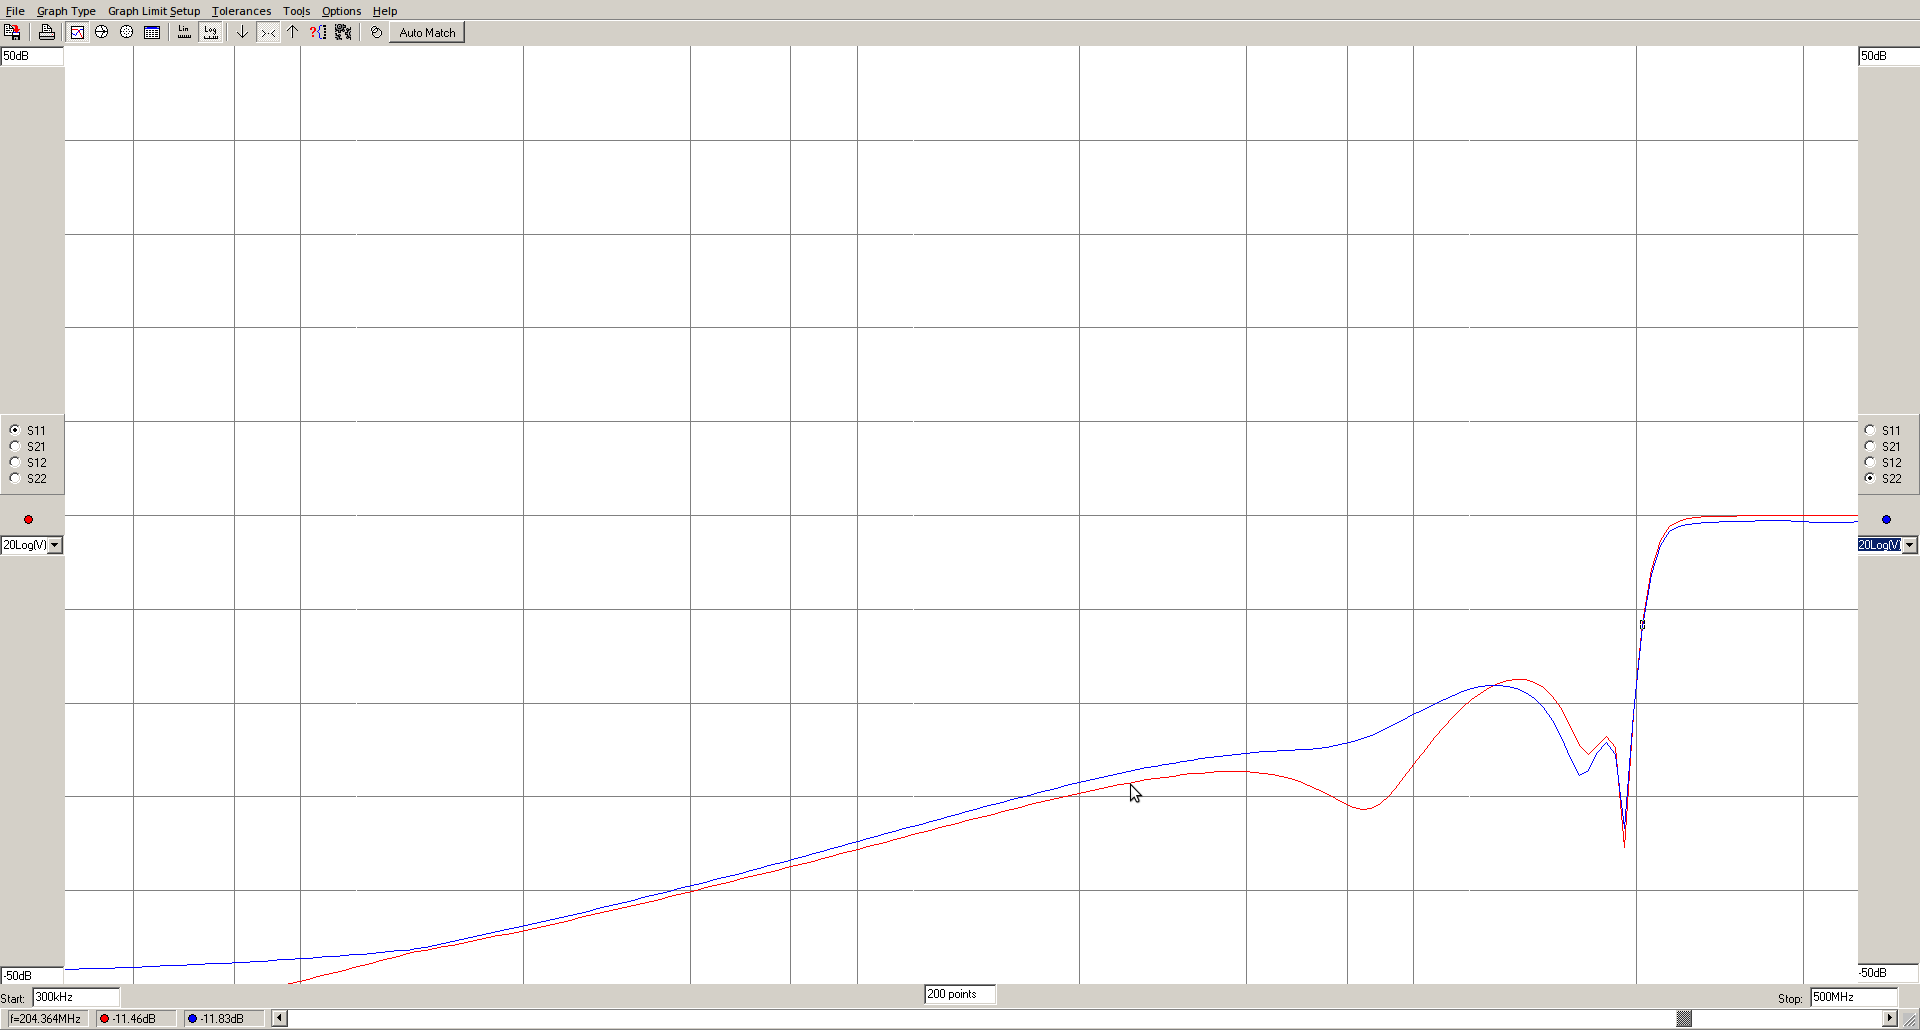
\includegraphics[scale = 0.25]{pic/reflexion_pb.png}\\ \end{center}
Cependant on peut remarquer que aux alentours de la fréquence de coupure les deux courbes sont réellement superposé
On peut aussi remarquer que l'on a une adaptation convenable, puisque nous sommes au maximum à -20dB en
ce qui concerne la bande passante du filtre.
\begin{center}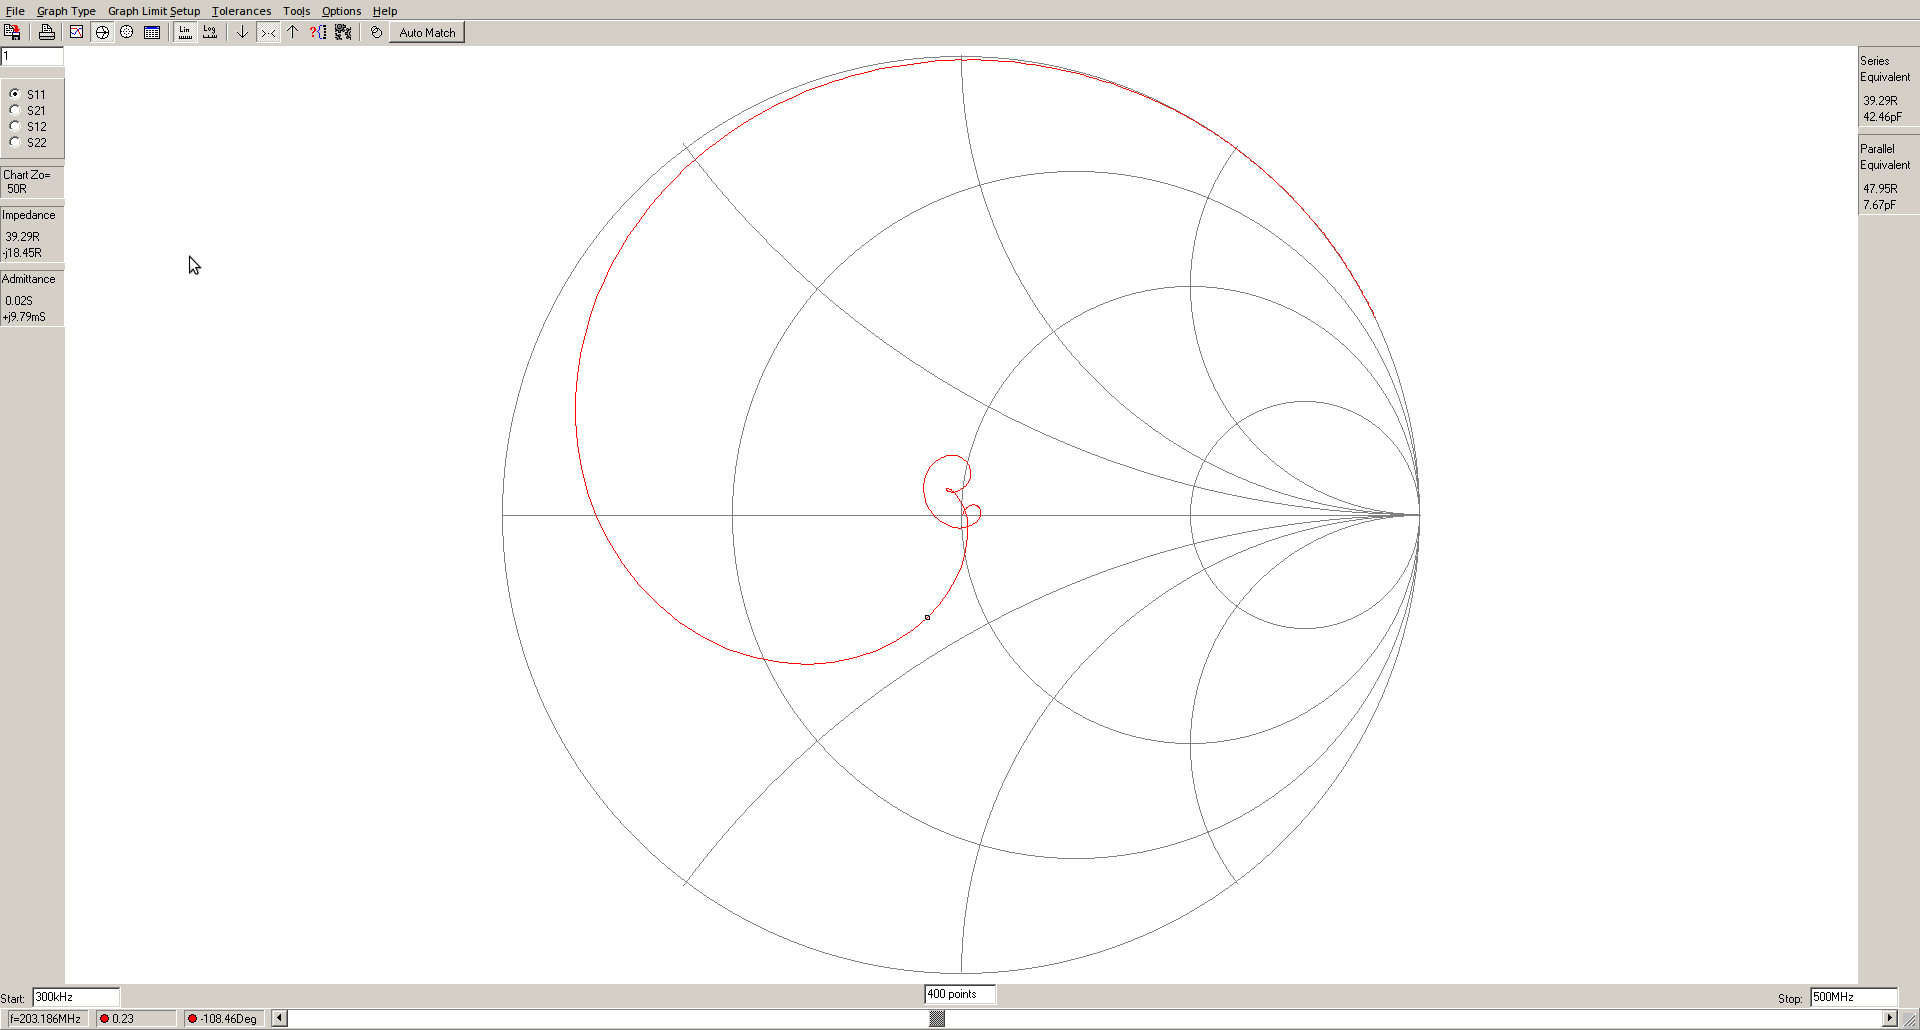
\includegraphics[scale = 0.25]{pic/Abaque_pb.png}\\ \end{center}
Sur ce graphique (Abaque) on peut y trouver l'impédence à la fréquence de coupure du filtre passe bas.
Qui est de 39,29R-j18,45 pour S11. Et de 35,17R-j12,39 pour S22
\begin{center}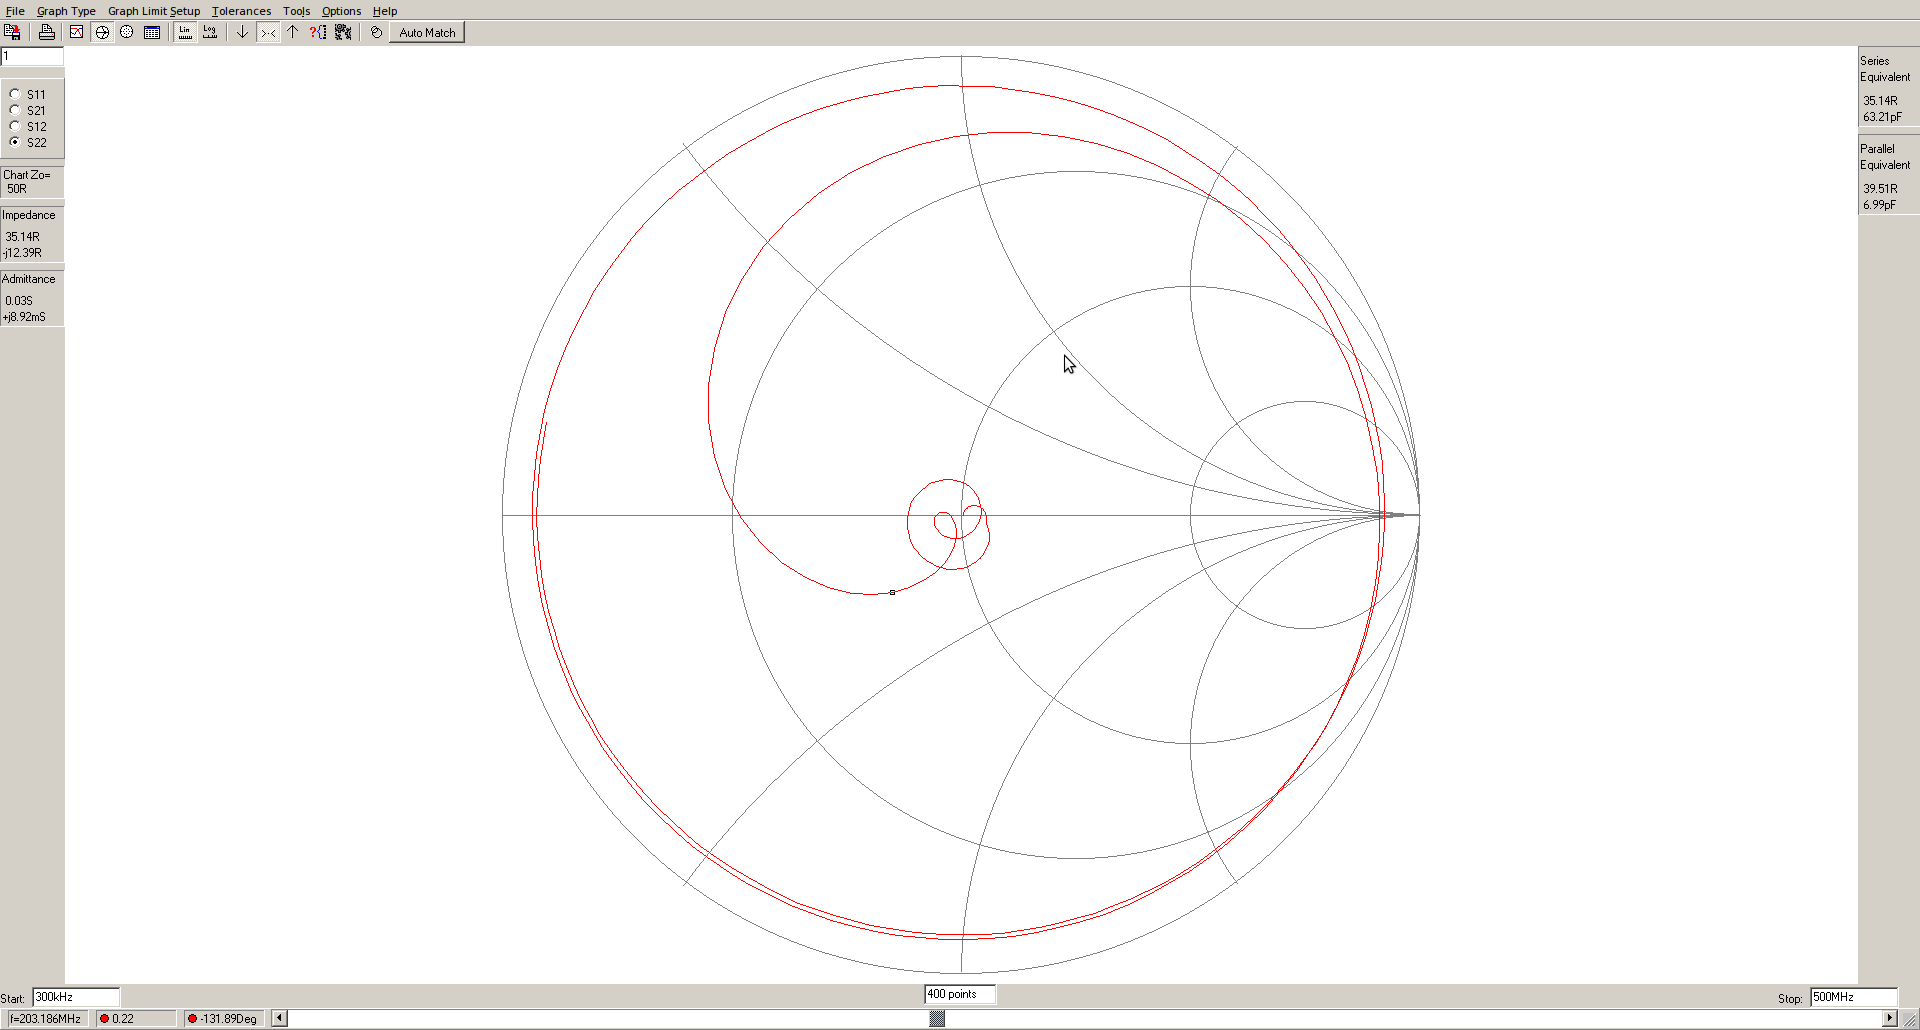
\includegraphics[scale = 0.25]{pic/Abaque_pbS22.png}\\ \end{center}
Et de 35,17R-j12,39

\section{Passe haut}

\begin{center}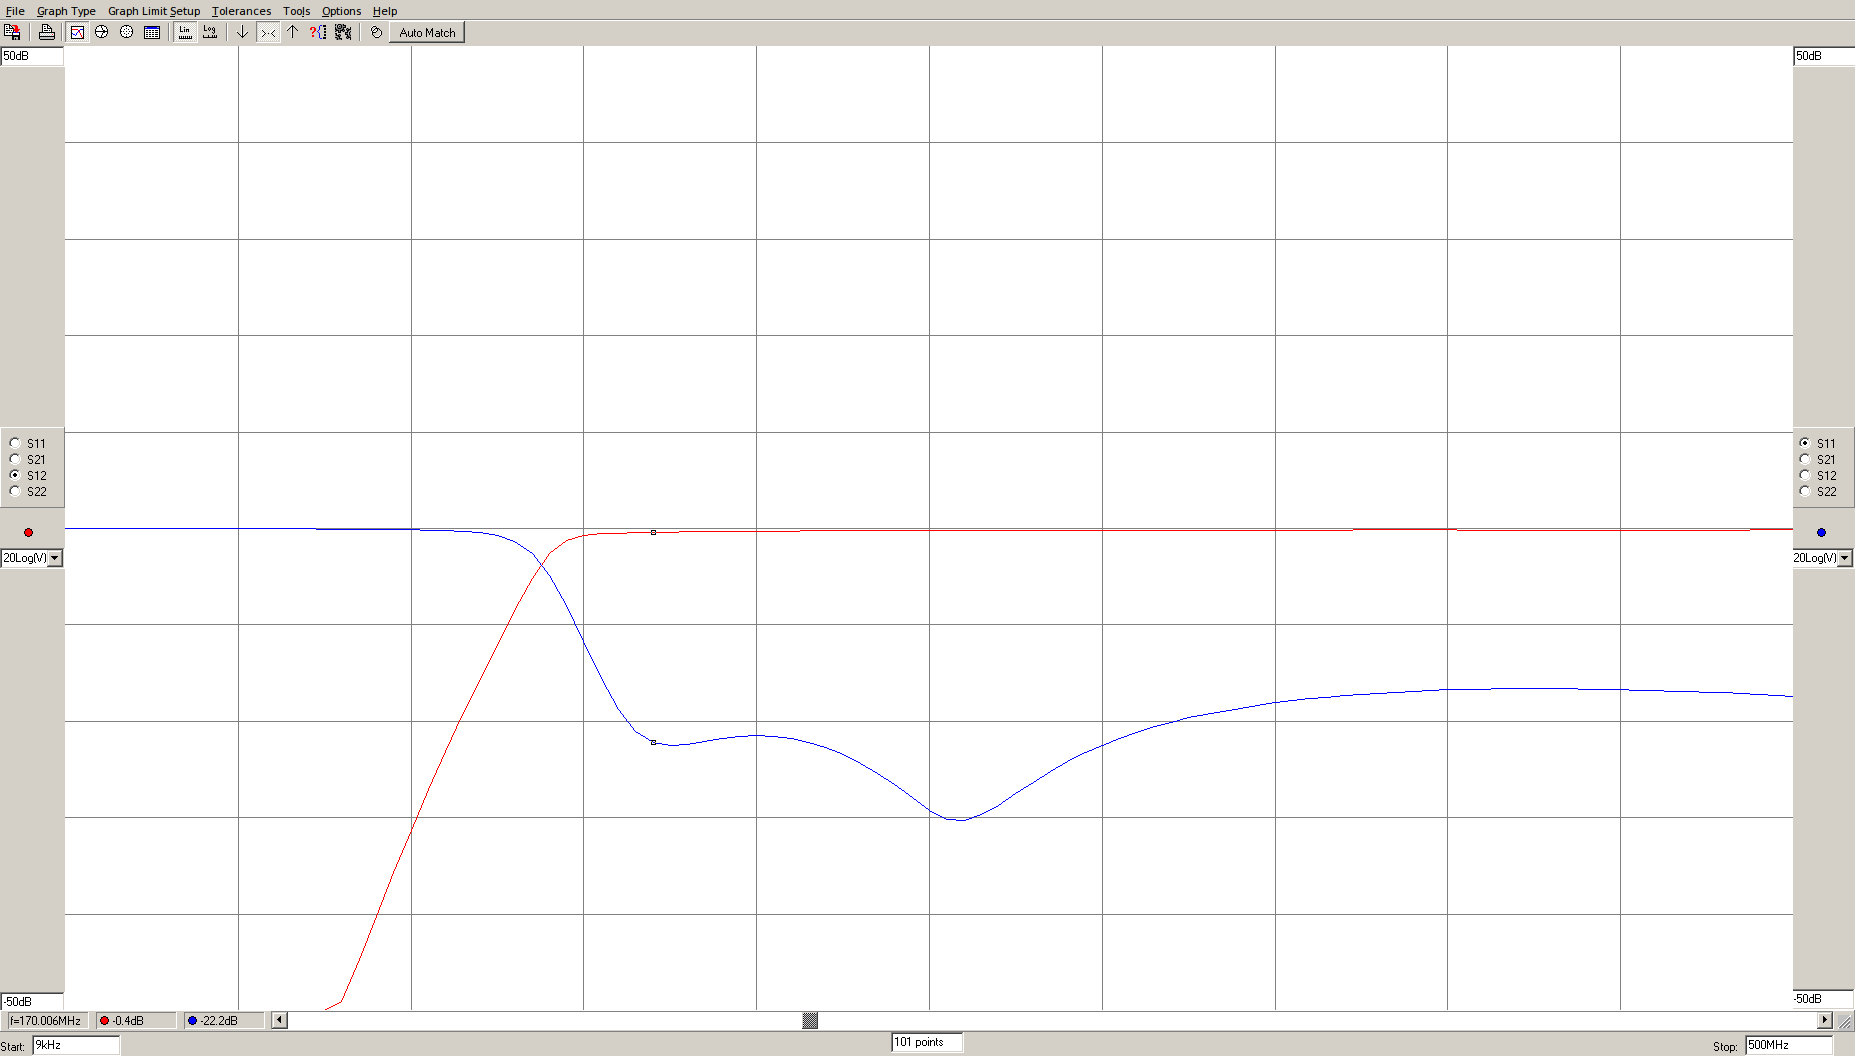
\includegraphics[scale = 0.25]{pic/parametre_passe_haut.png}\\ \end{center}
De la même façon que pour le passe bas, on distingue facilement qu'il sagit d'un passe haut.
Avec toujours en rouge la transmission (S12) ten bleu l'adaptation (S11). Pour le passe haut 
on a donc une fréquence de coupure à -1dB de 147.992MHz.
\begin{center}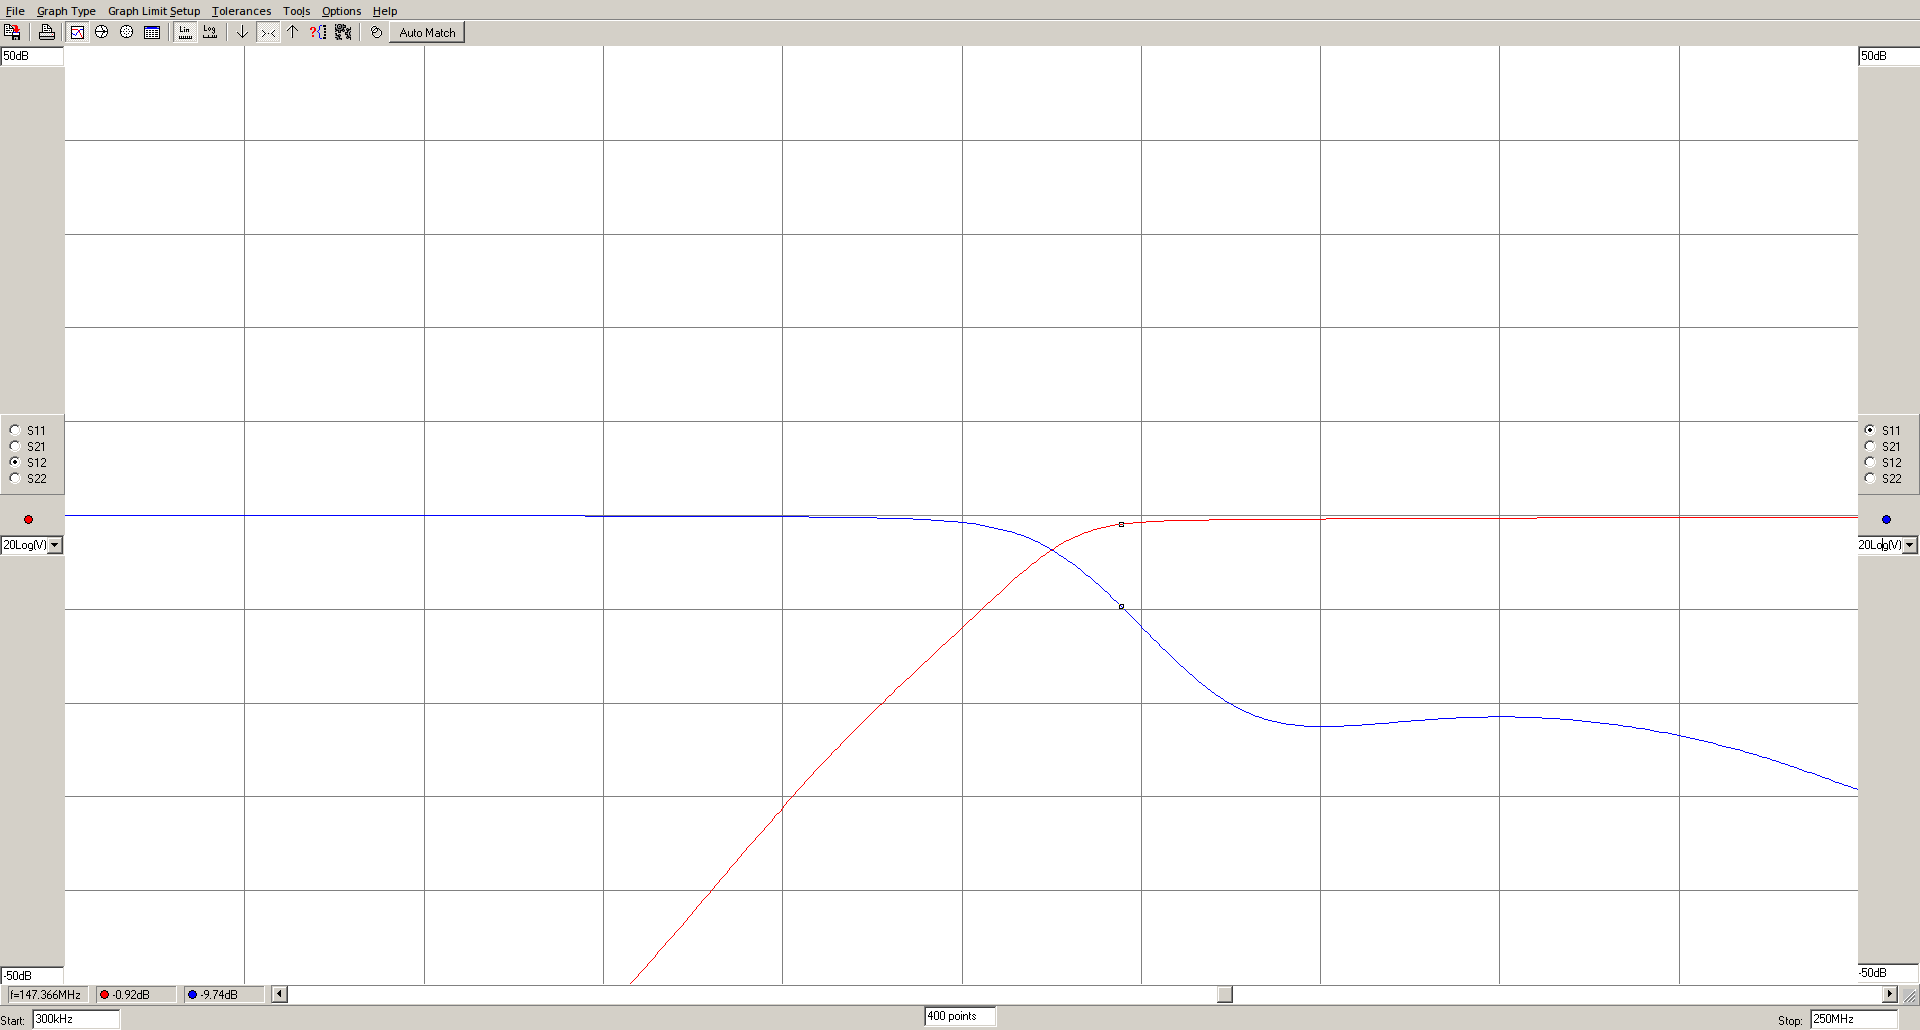
\includegraphics[scale = 0.25]{pic/freq_coupure_ph.png}\\ \end{center}

\begin{center}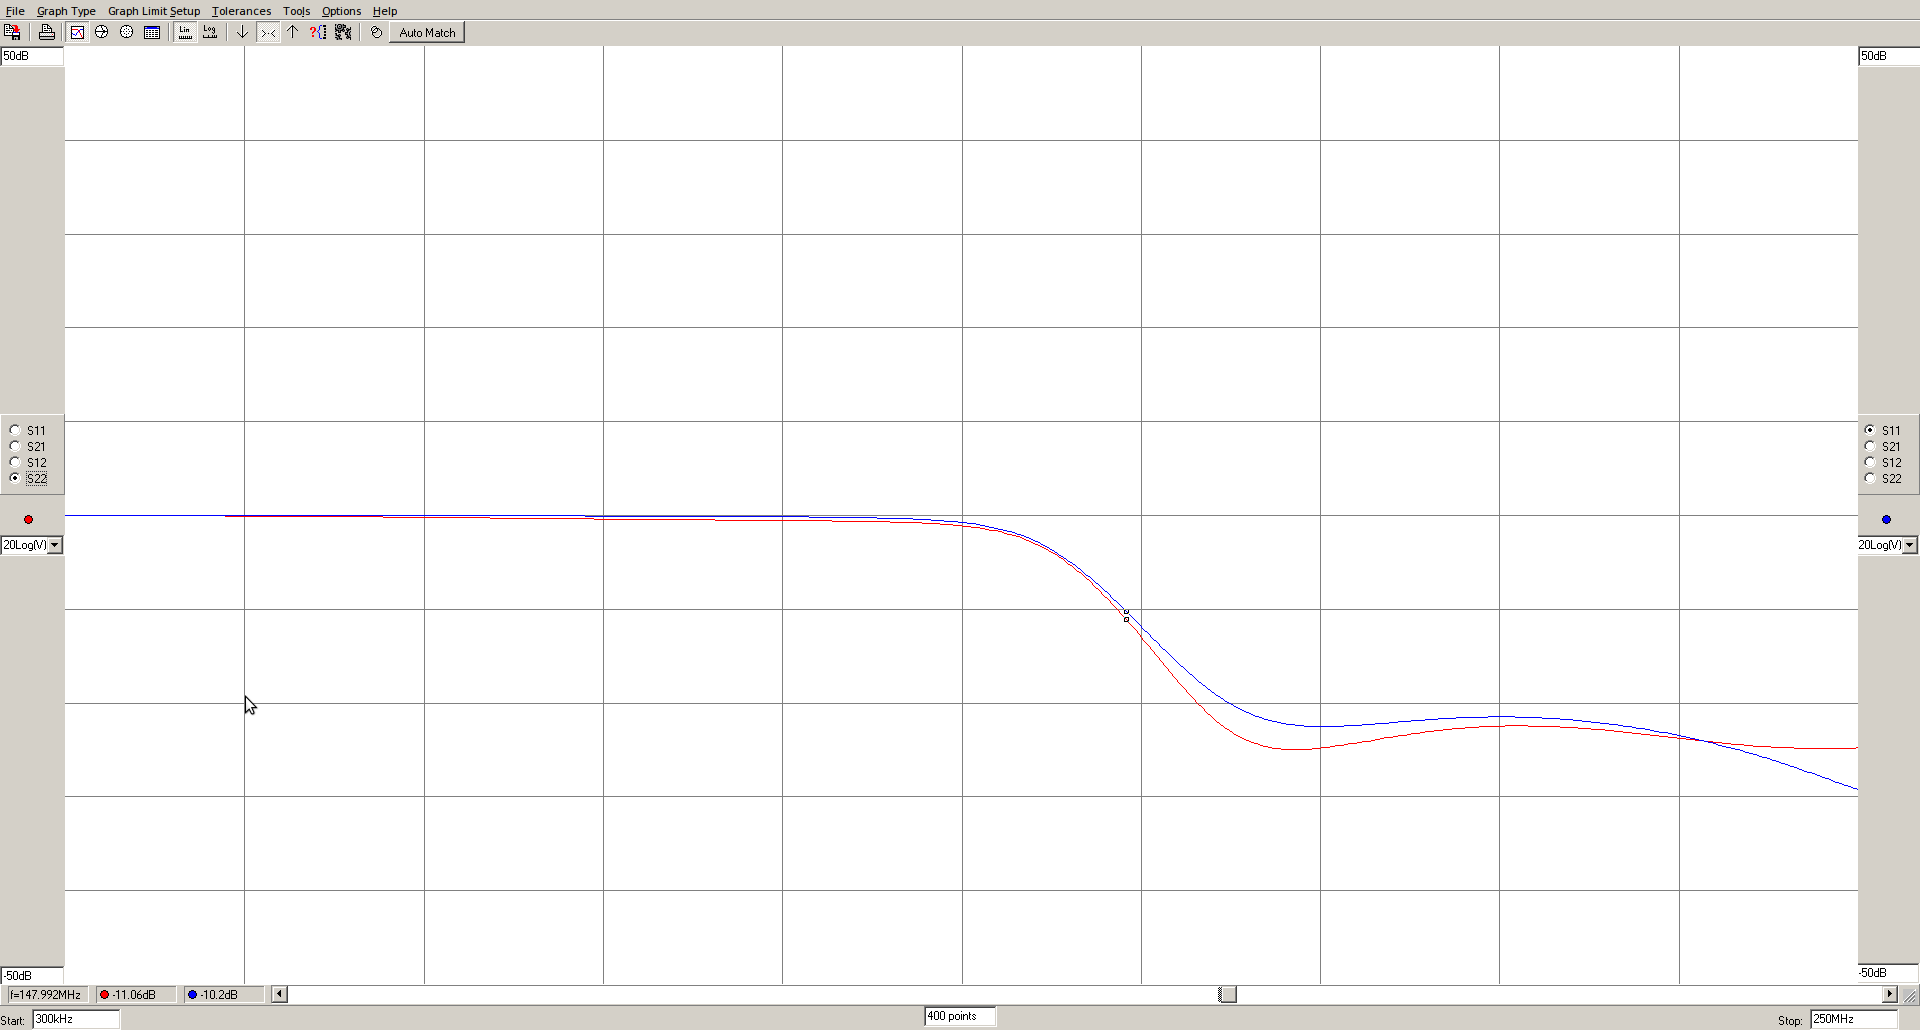
\includegraphics[scale = 0.25]{pic/reflexion_ph.png}\\ \end{center}
Pour le passe haut on peut voir que les deux courbes de réflexions ne sont pas tout à fait 
identique au niveau de la fréquence de coupure -11,6dB pour S22 et -10.2dB pour S11. Cependant 
elles se suivent parfaitement et l'adaptation et suffisante puisque l'on reste en dessous des -10dB.

\begin{center}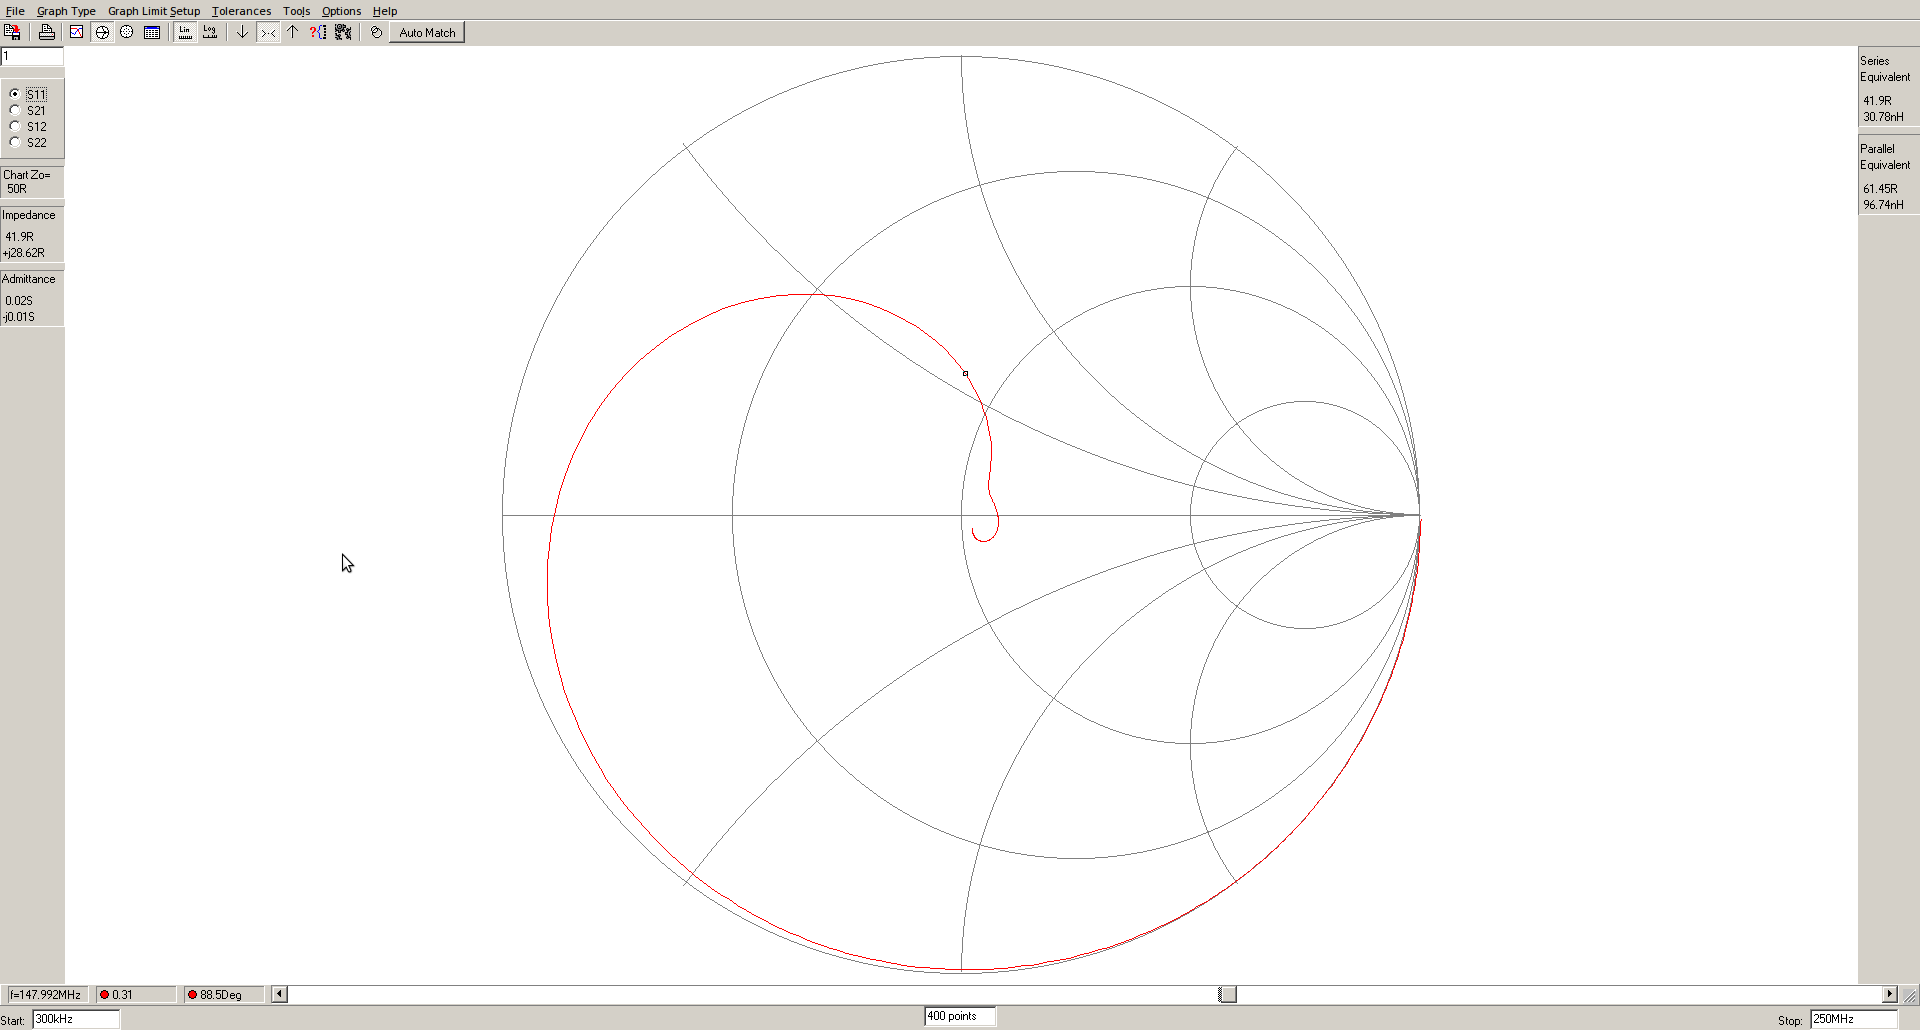
\includegraphics[scale = 0.25]{pic/abaque_phs11.png}\\ \end{center}
Pour S11 nous avons une impédence de 41,9R+j28,62 à 147,992MHz.

\begin{center}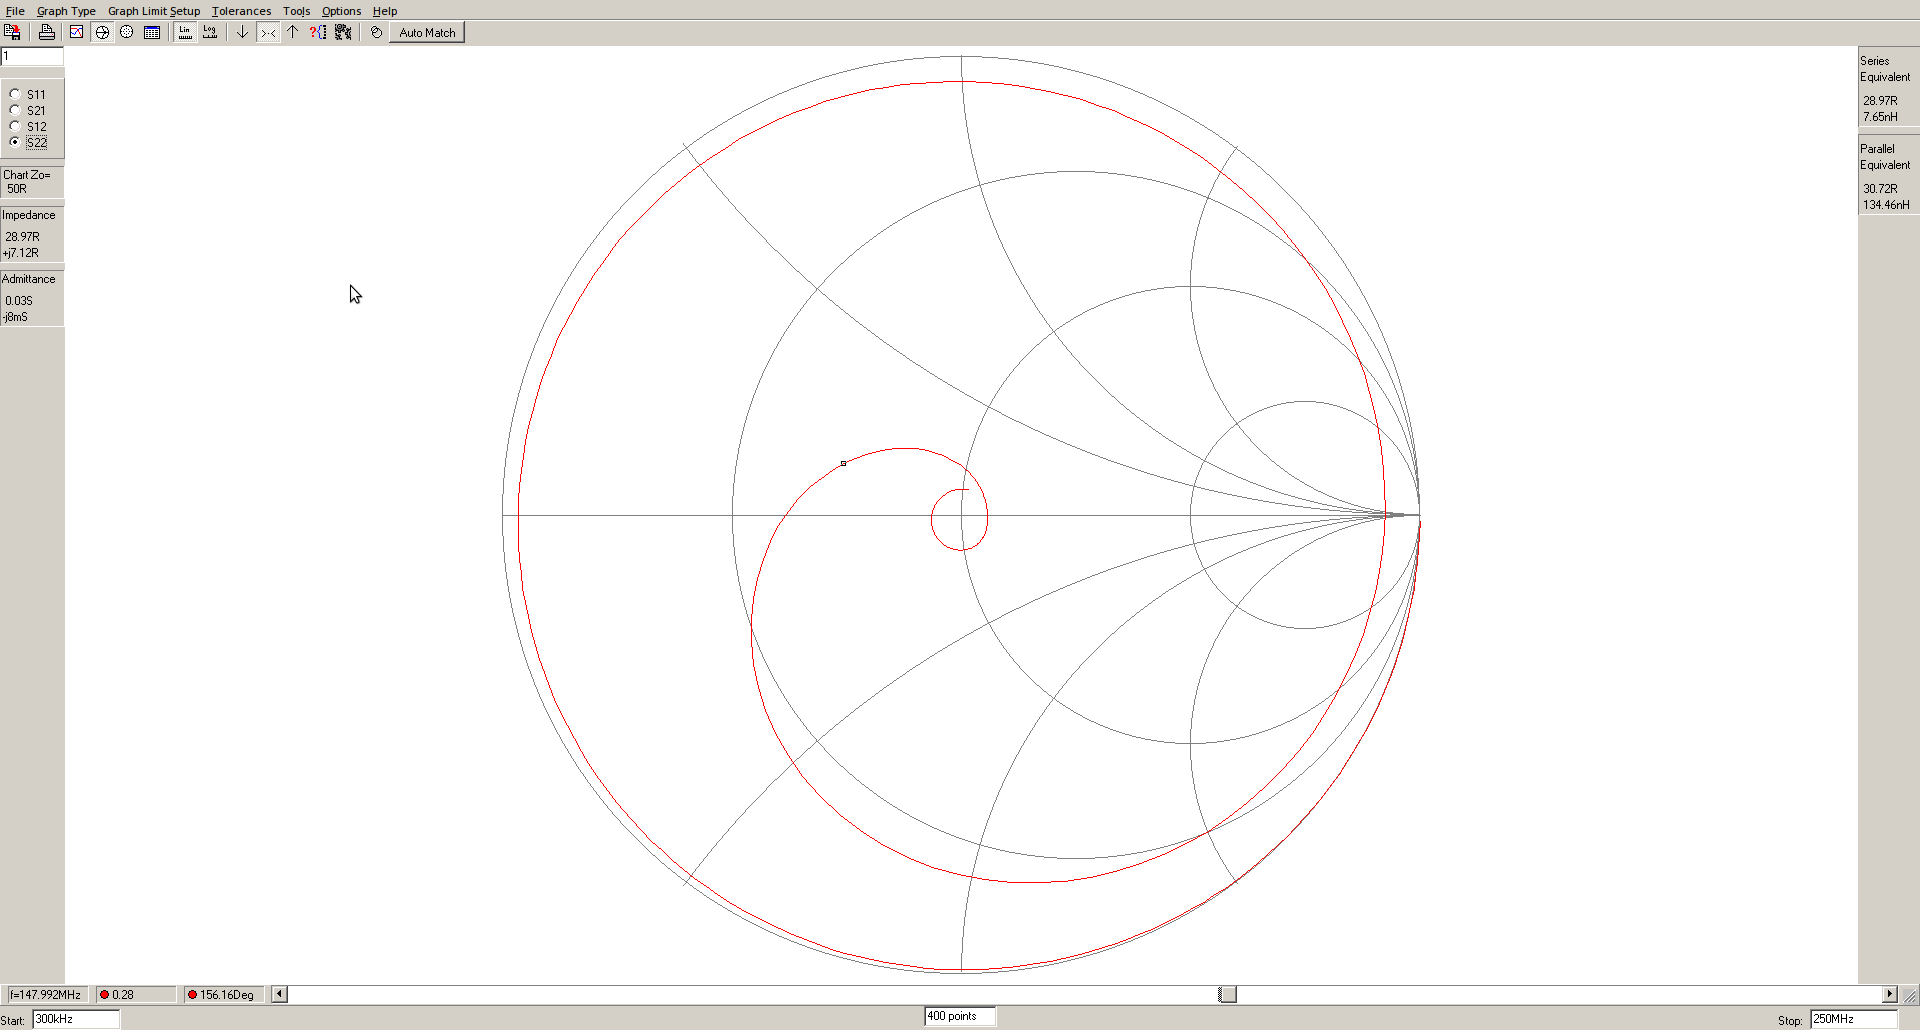
\includegraphics[scale = 0.25]{pic/abaque_phs22.png}\\ \end{center}
Pour S22 nous avons une impédence de 28,97R+j7,12 à 147,992MHz.

\chapter{Association des filtres}
\addcontentsline{toc}{chapter}{Association des filtres}

\section{Cablage}

\begin{center}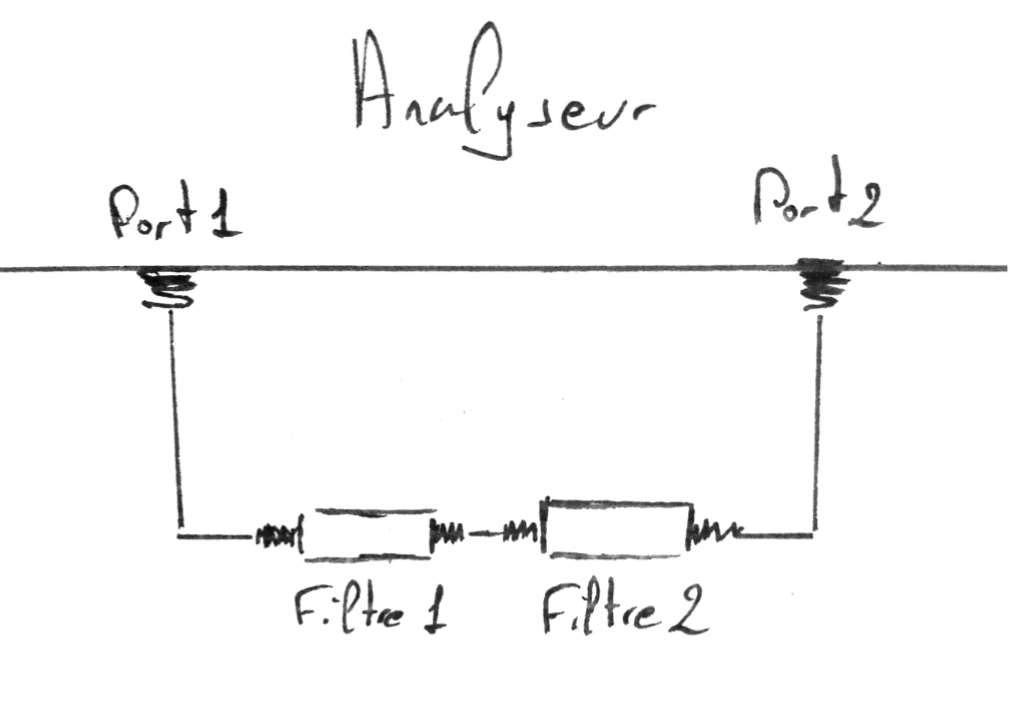
\includegraphics[scale = 0.2]{pic/Cablage_filtre2.png}\\ \end{center}
Pour l'association des filtres nous avons juste brancher les deux filtre ensemble. 
Le passe haut et le passe bas, ce qui devrait créer un passe bande. Il ne restera plus
qu'à trouver sont type.
\newpage
\section{Mesures}

\begin{center}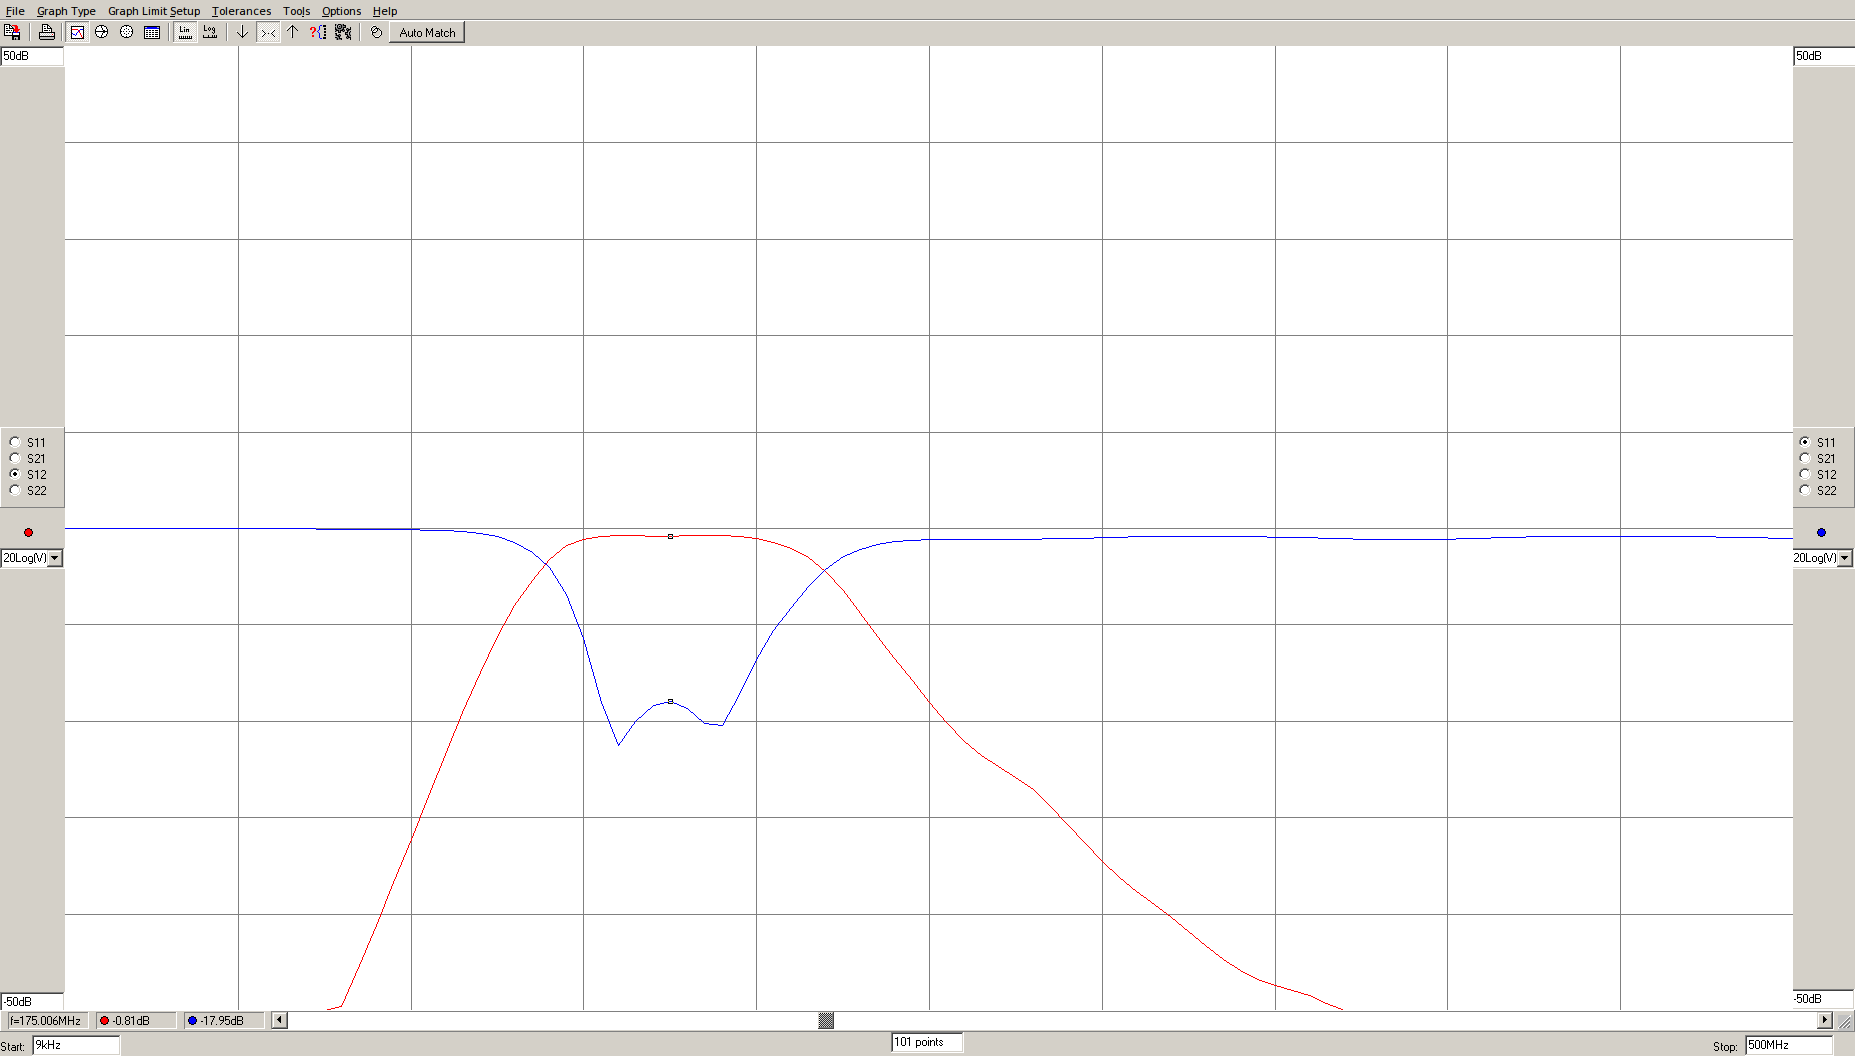
\includegraphics[scale = 0.25]{pic/parametre_passe_bande.png}\\ \end{center}
Lors de nos relevé la bande passante à -3dB est de 75,143MHz (215,71MHz-140,567MHz). 
La bande passante à -40dB est de 226,681MHz (91,724MHz-318,405MHz). Lors des mesures pour
le passe bas et le passe haut nous n'avons décelé aucune ondulation. Ainsi il semble normal 
de ne toruver aucune ondulation pour le passe bande. Puisqu'il est composé du passe haut et
du passe bas étudier précédement.
Les pertes d'insertions sont quant-à-elle faible puisque l'on est à -0.75dB, en prenant compte
la calibration à bien été faite et minimise la perte liée au cable et au connecteur.
Toute ces mesures sont facilement réalisable grâce à rfsim99 et on pour but de déterminer
le type, la famille du filtre butterworth ou tchebychev.\\
Ce filtre est donc un filtre passe bande butterworth, on peut le remarquer grâce aux pentes 
qui ne sont pas raide et en l'absence d'ondulation. 


\chapter{Diviseur de puissance}
\addcontentsline{toc}{chapter}{Diviseur de puissance}

\begin{center}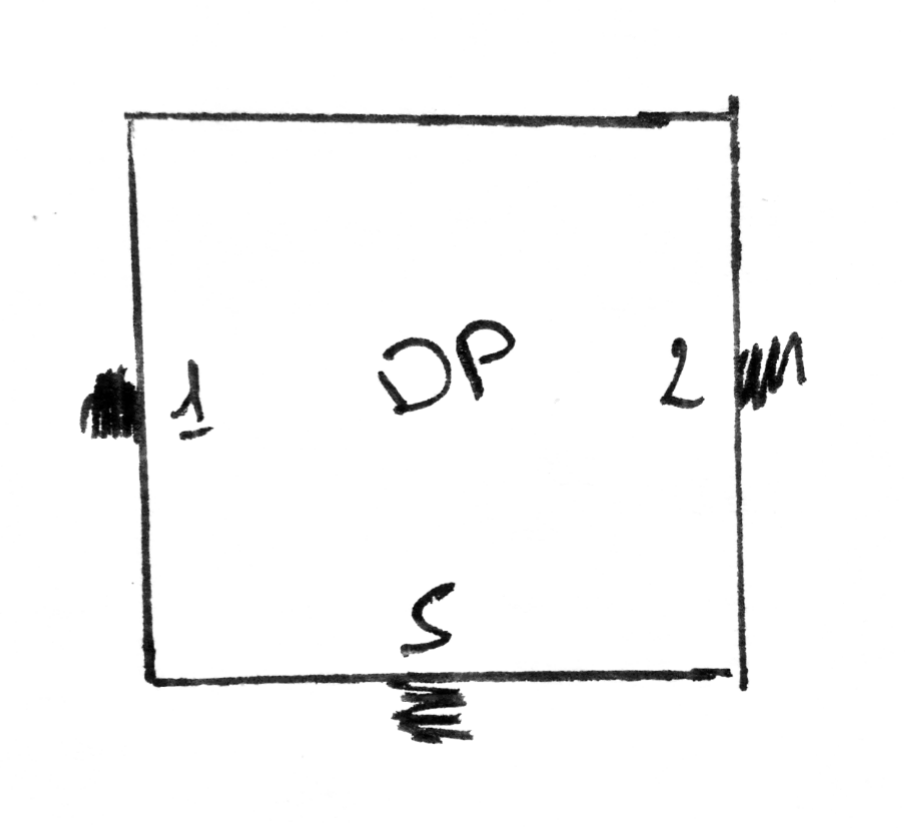
\includegraphics[scale = 0.2]{pic/DP.png}\\ \end{center}

\section{Transmission \& Adaptation}

\subsection{Cablage}
\begin{center}
	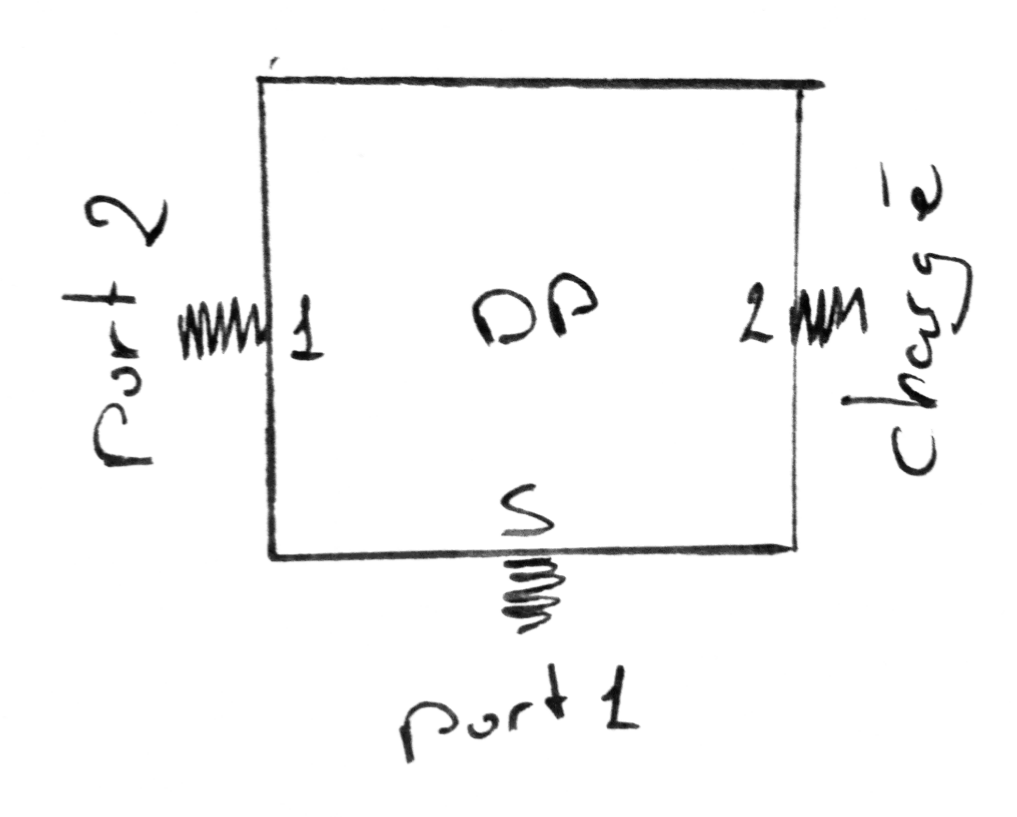
\includegraphics[scale = 0.15]{pic/DPS1.png}
      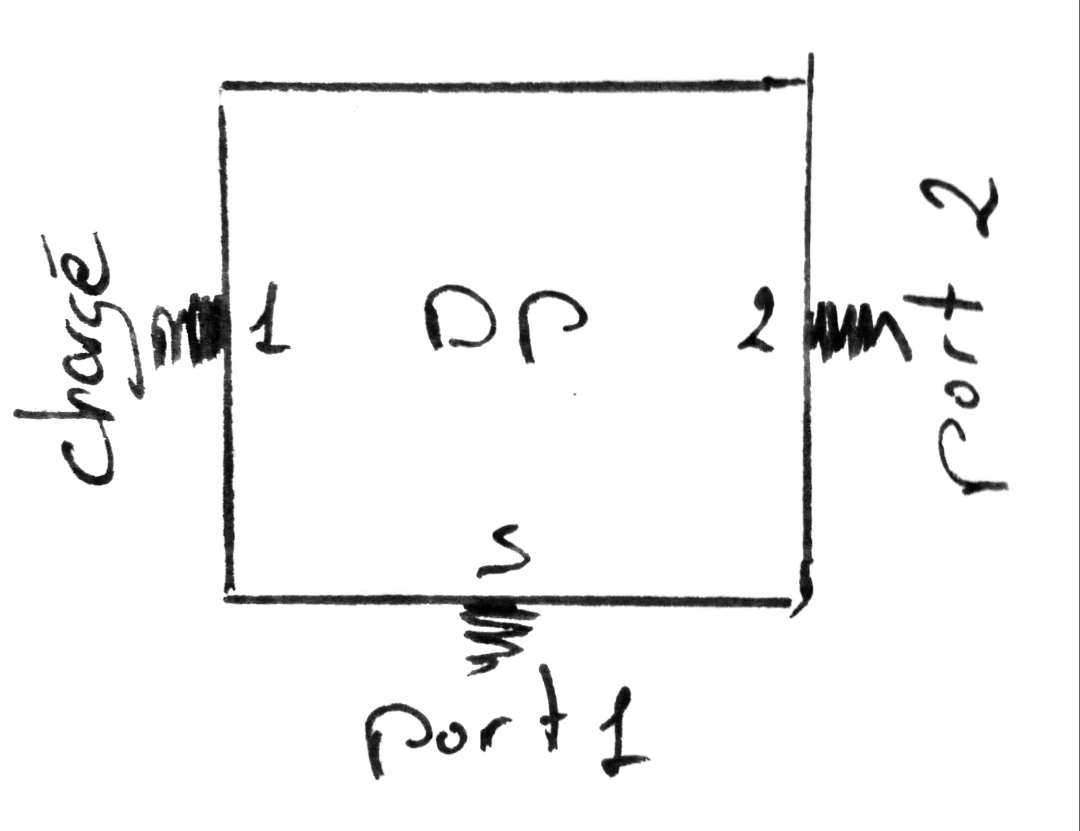
\includegraphics[scale = 0.15]{pic/DPS2.png}
\end{center}
Tout port qui n'est pas relié à l'analyseur sera brancher à une charge de 50ohm.
\newpage
\subsection{Mesures}
\begin{center}
	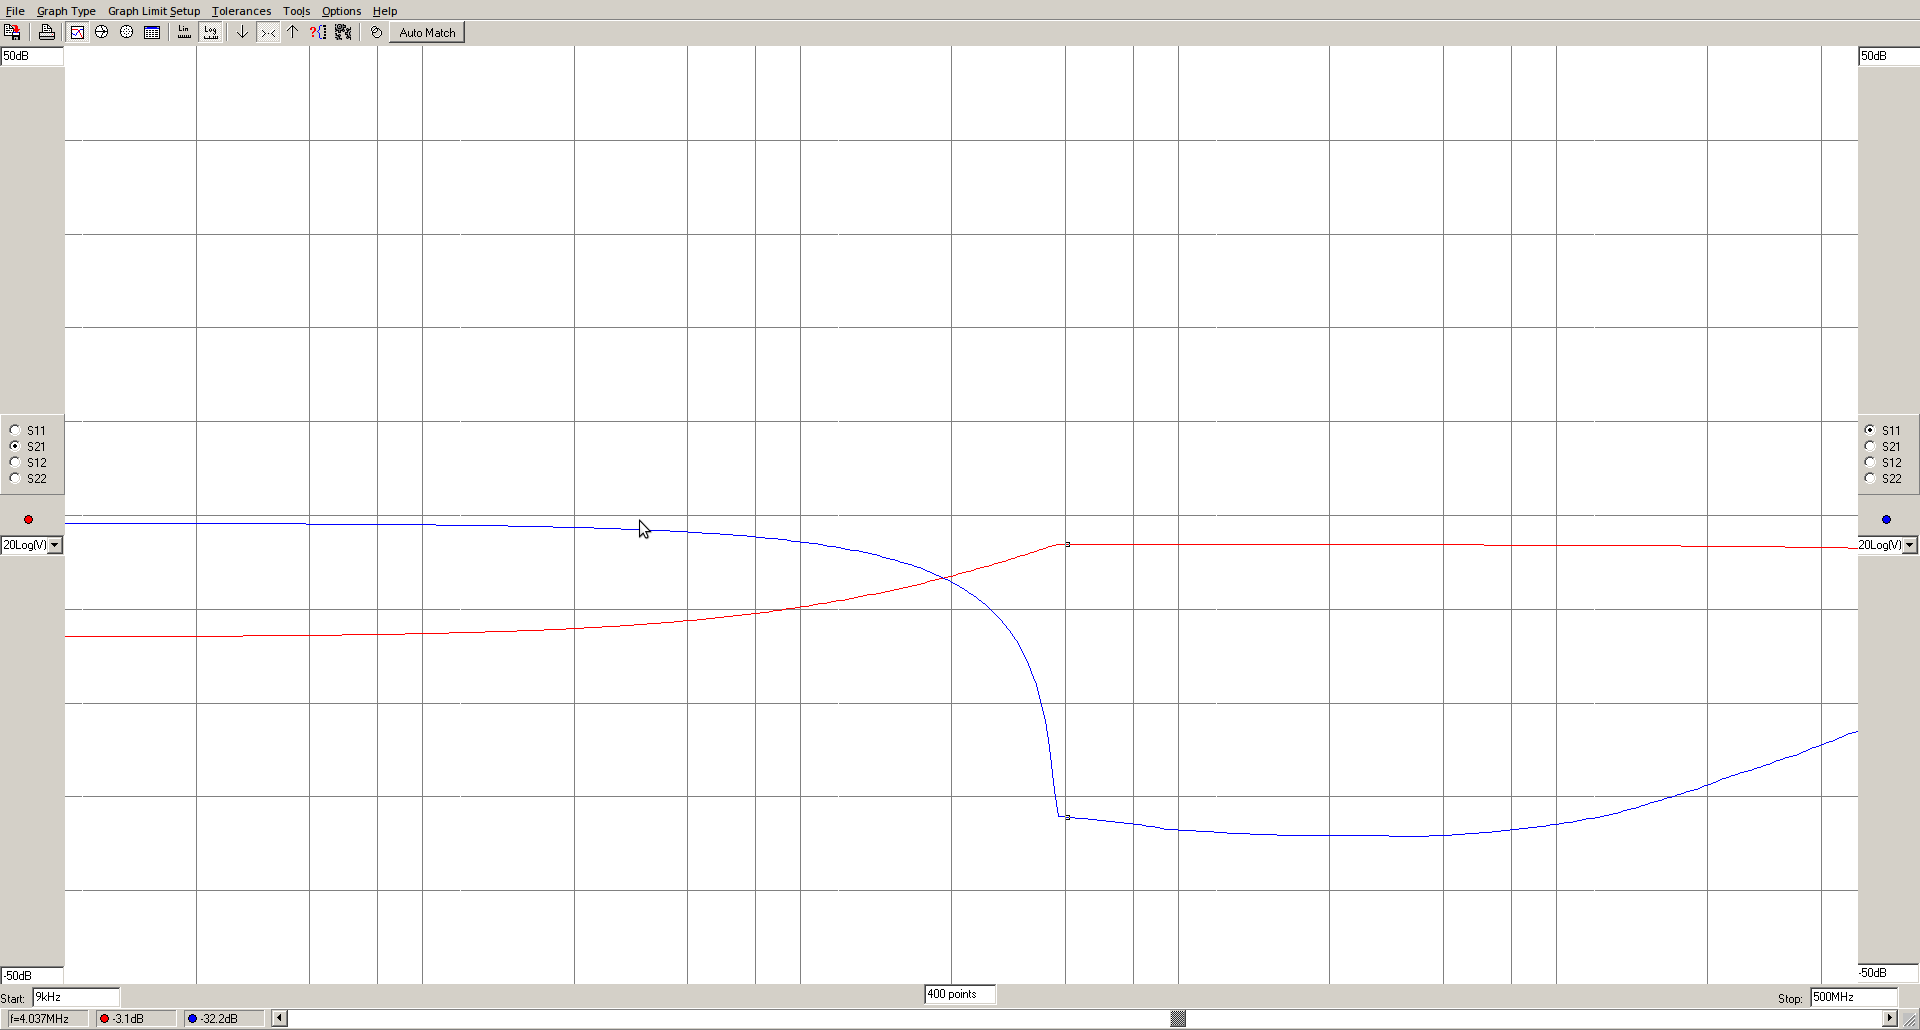
\includegraphics[scale = 0.25]{pic/div_ps1.png} \\
	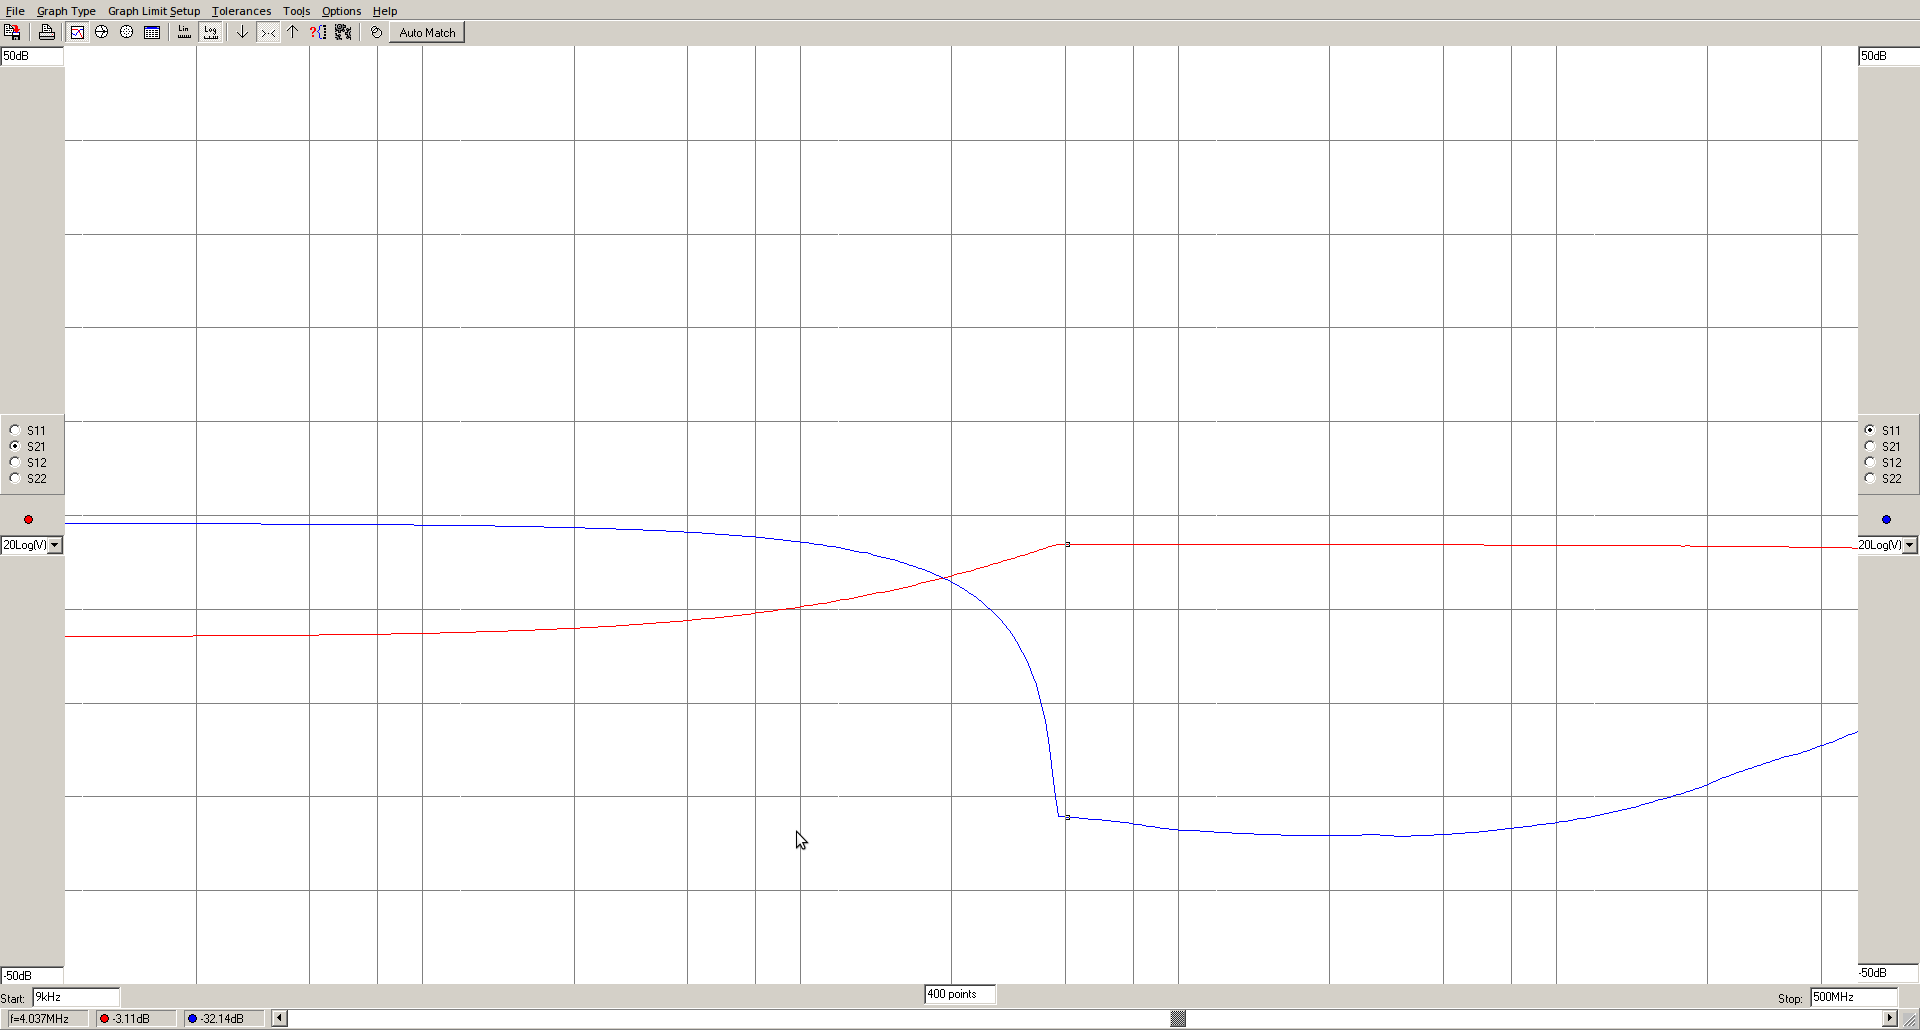
\includegraphics[scale = 0.25]{pic/div_ps2.png}
\end{center}
On peut donc voir respectivement ci-dessus, le diviseur de puissance branché de :
S vers 1 et S vers 2. Le composant étant symetrique et passif il est normal de retrouver
exactement la même chose pour les deux. A savoir une atténuation de 3dB parfaitement linéaire
à partir de 4MHz avec une bonne adaptation de -32dB.
\section{Isolation}
\subsection{Cablage}

\begin{center}
	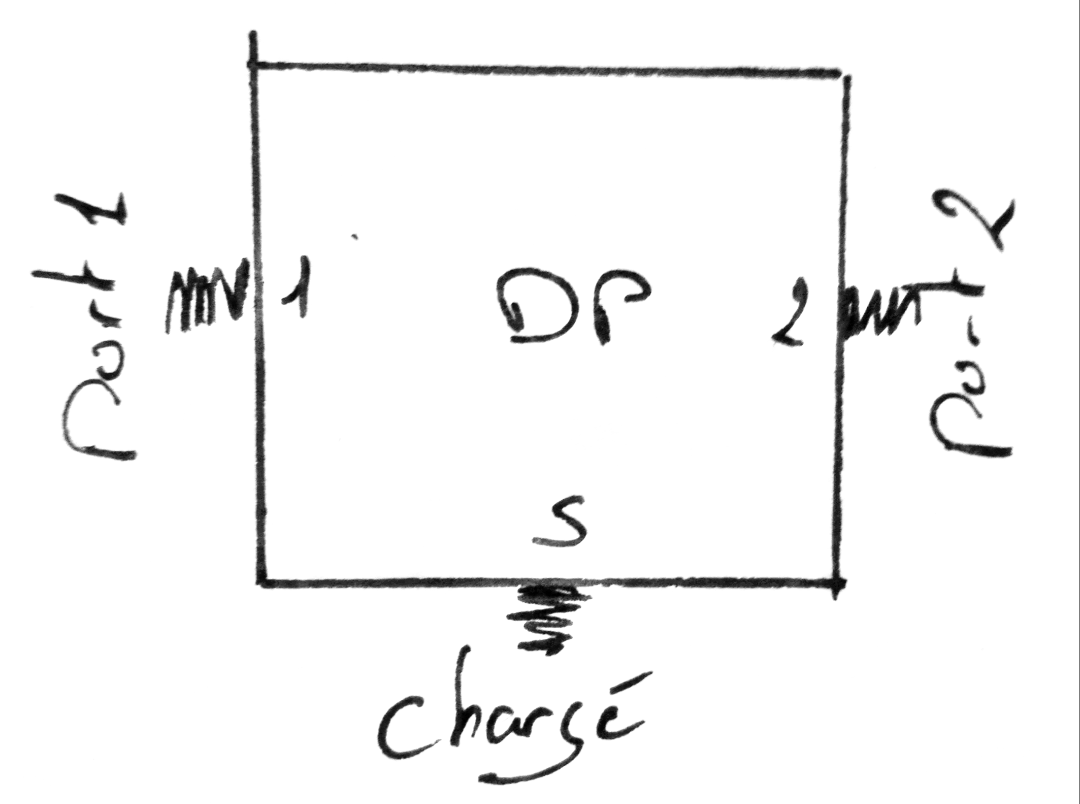
\includegraphics[scale = 0.15]{pic/DP12.png} \\\end{center}

\subsection{Mesures}
\begin{center}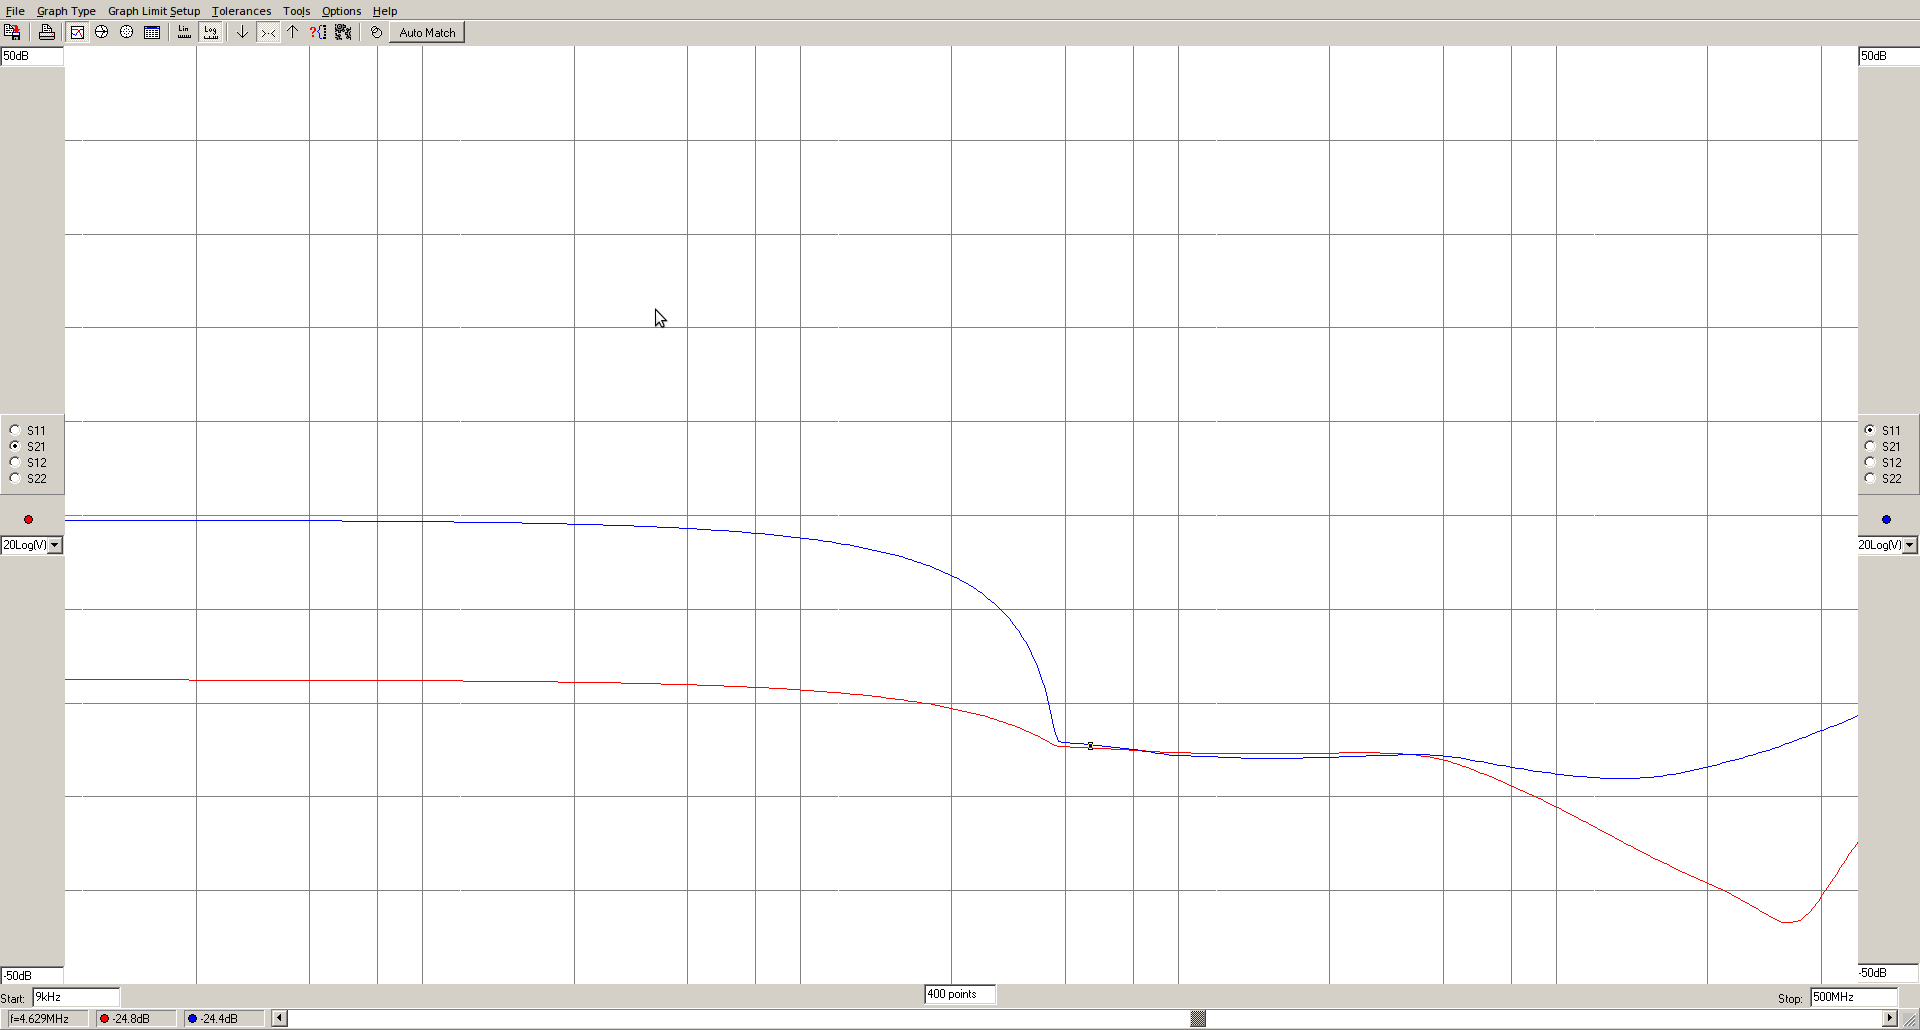
\includegraphics[scale = 0.25]{pic/isolation_dp12.png}\\ \end{center}
On peut voir que l'isolation (en rouge) est suffisante entre le port 1 et 2 puisque on se trouve systématiquement
en dessous de l'adaptation (en bleu)

\chapter{Coupleur directif}
\addcontentsline{toc}{chapter}{Coupleur directif}
\begin{center}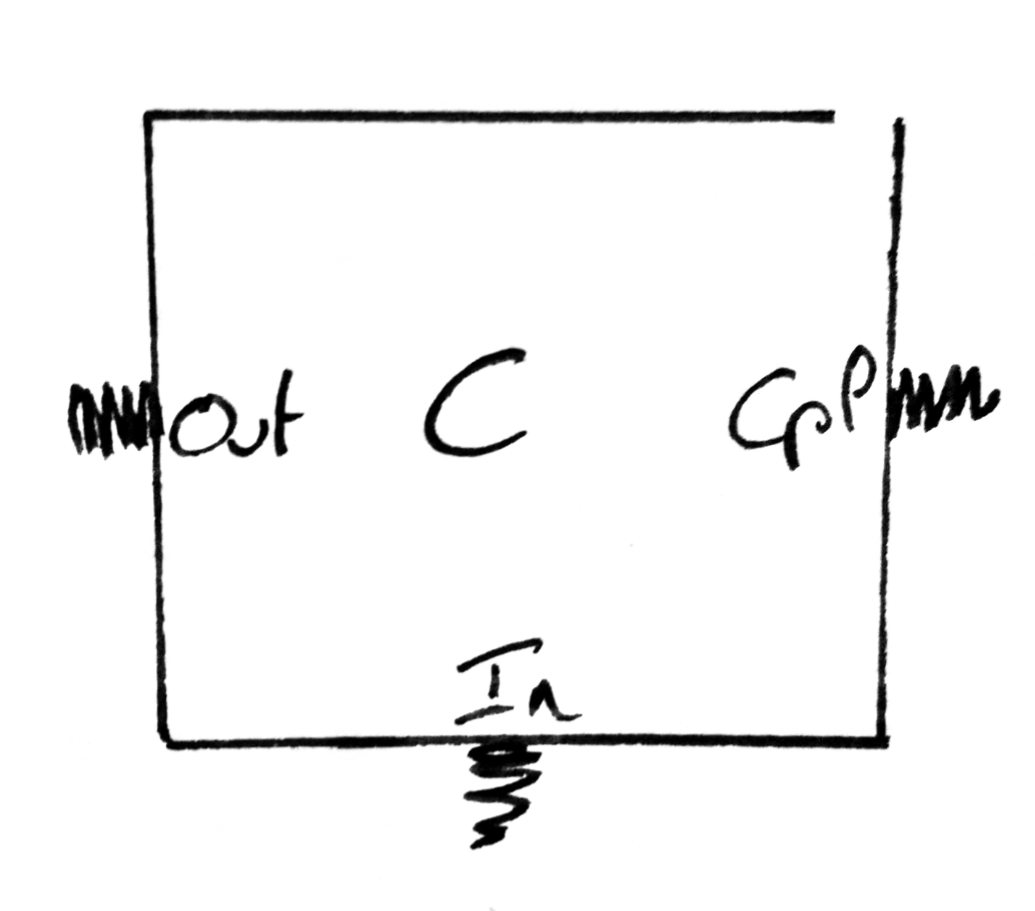
\includegraphics[scale = 0.17]{pic/CD.png}\\ \end{center}

\section{Transmission}
\subsection{Cablage}
\begin{center}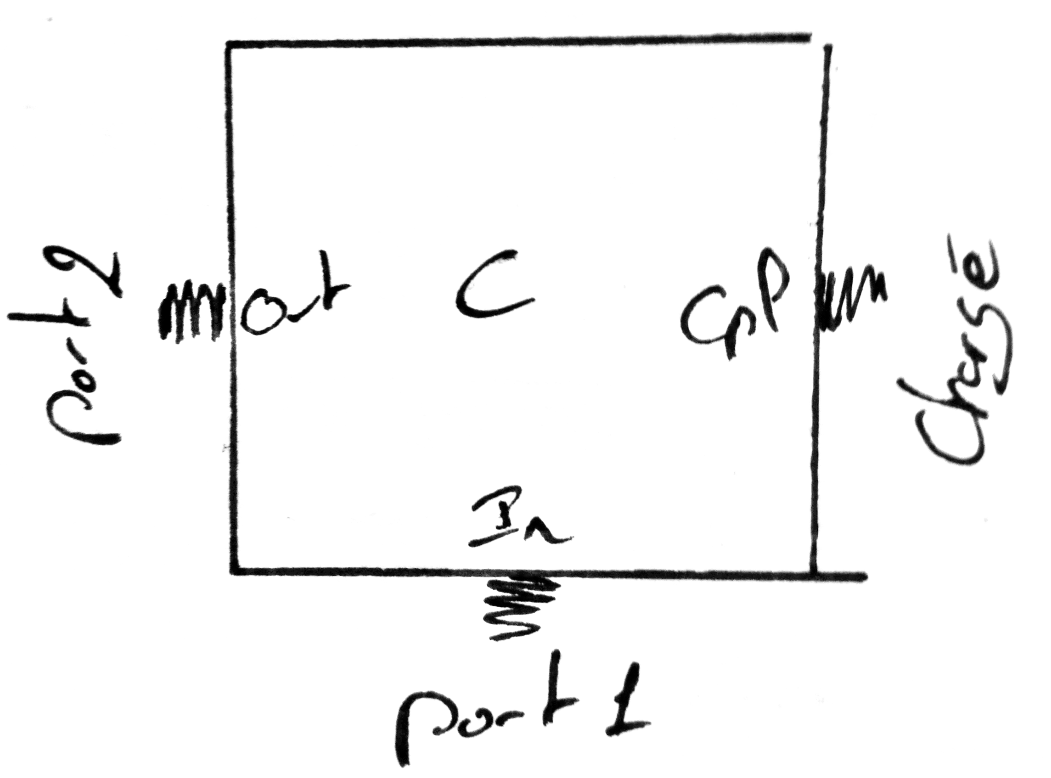
\includegraphics[scale = 0.17]{pic/CDIO.png}\\ \end{center}
De même que pour le diviseur de puissance, lors de nos tests tout port qui n'est pas branché
à l'analyseur sera chargé à 50ohm.
\newpage
\subsection{Mesures}
\begin{center}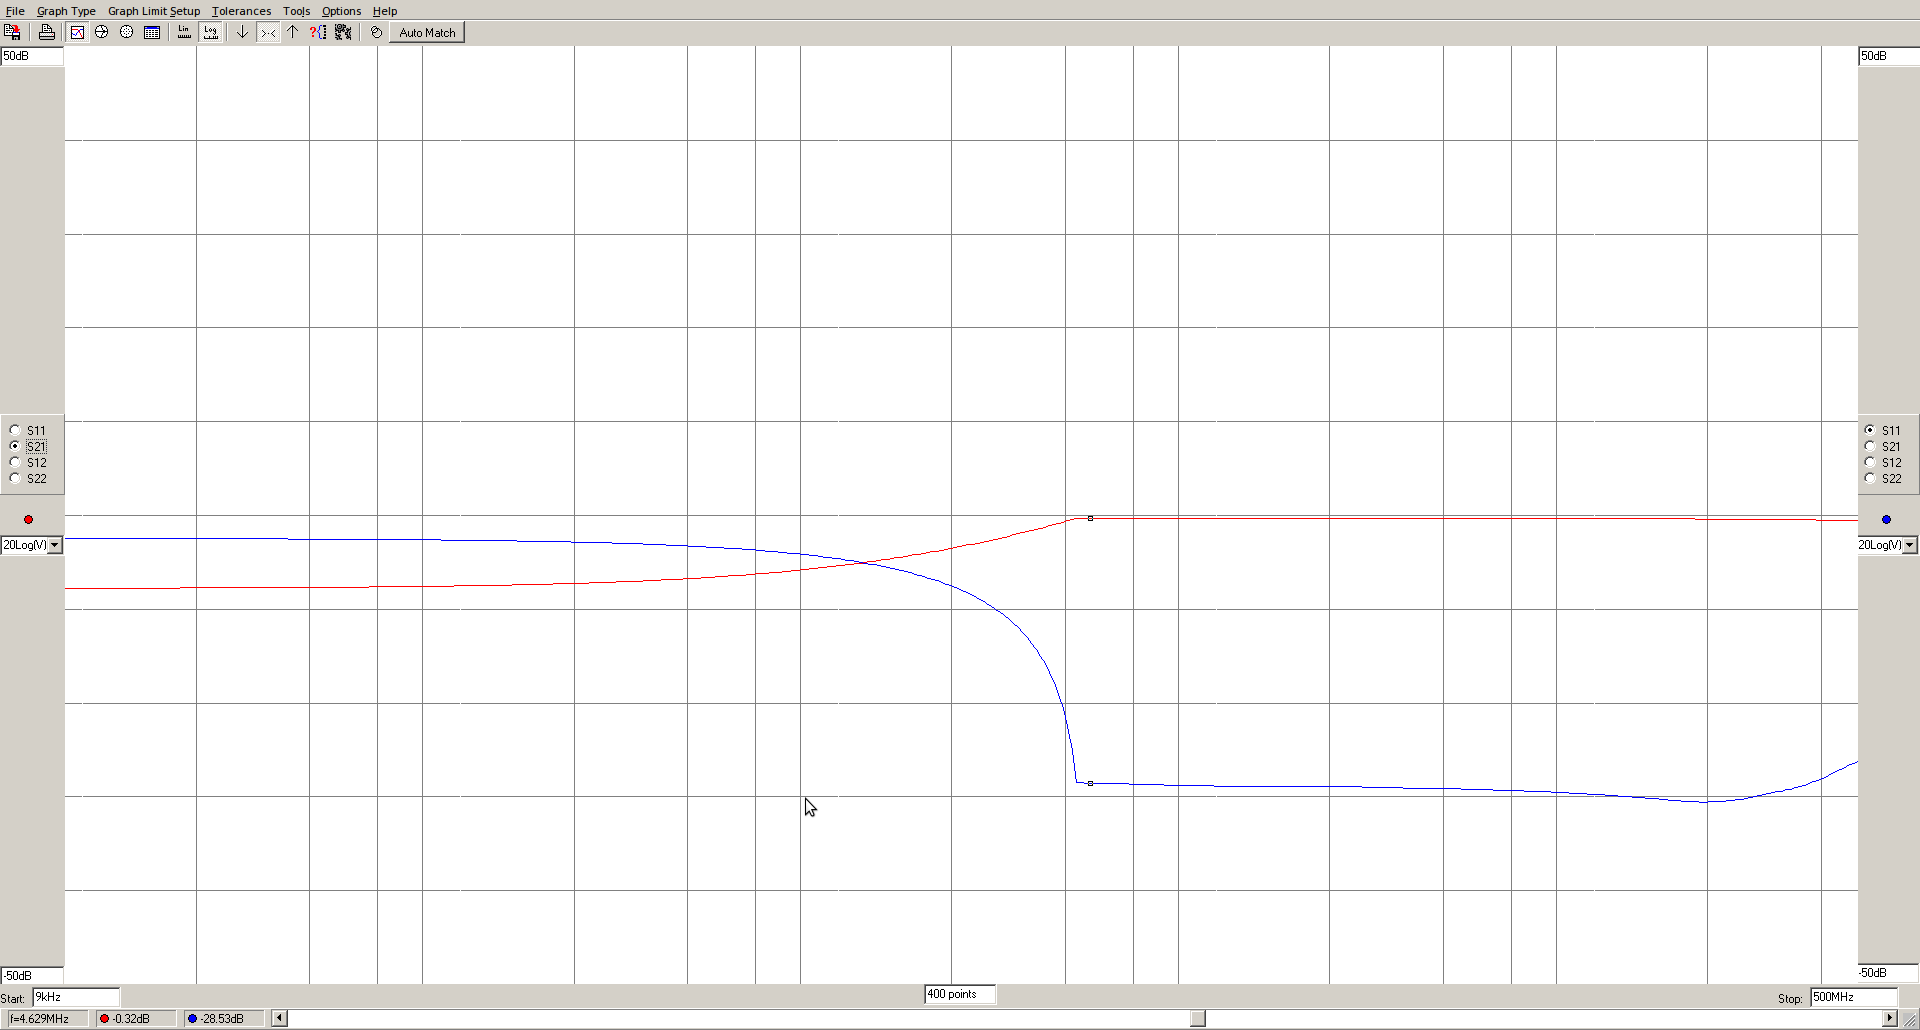
\includegraphics[scale = 0.25]{pic/cdio.png} \\ \end{center}
A l'aide de cette mesure on peut voir que une fois le système adapté (partie droite à -30dB), nous 
n'avons aucune perte du signal entre l'entrée et la sortie. Puisque l'on retrouve une transmission à
0dB dans cette partie.
\section{Couplage}
\subsection{Cablage}
\begin{center}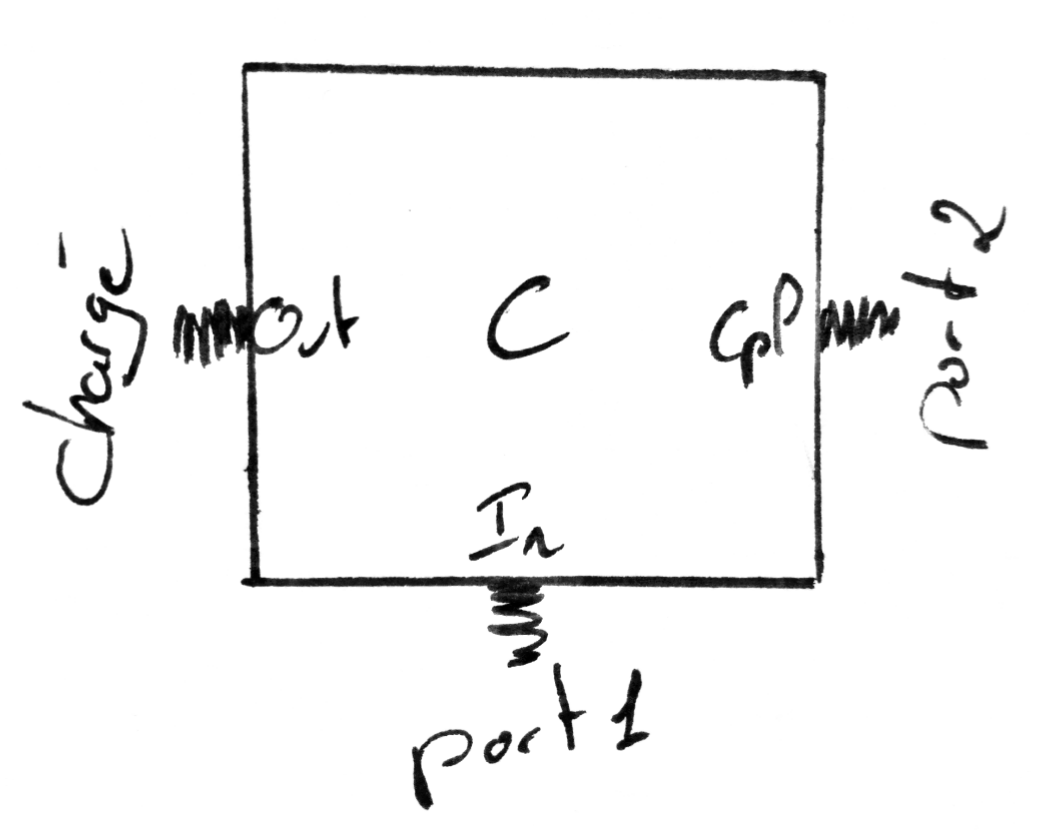
\includegraphics[scale = 0.17]{pic/CDIC.png}\\ \end{center}
De même que précédement tout port vide sera chargé.
\newpage 
\subsection{Mesures}
\begin{center}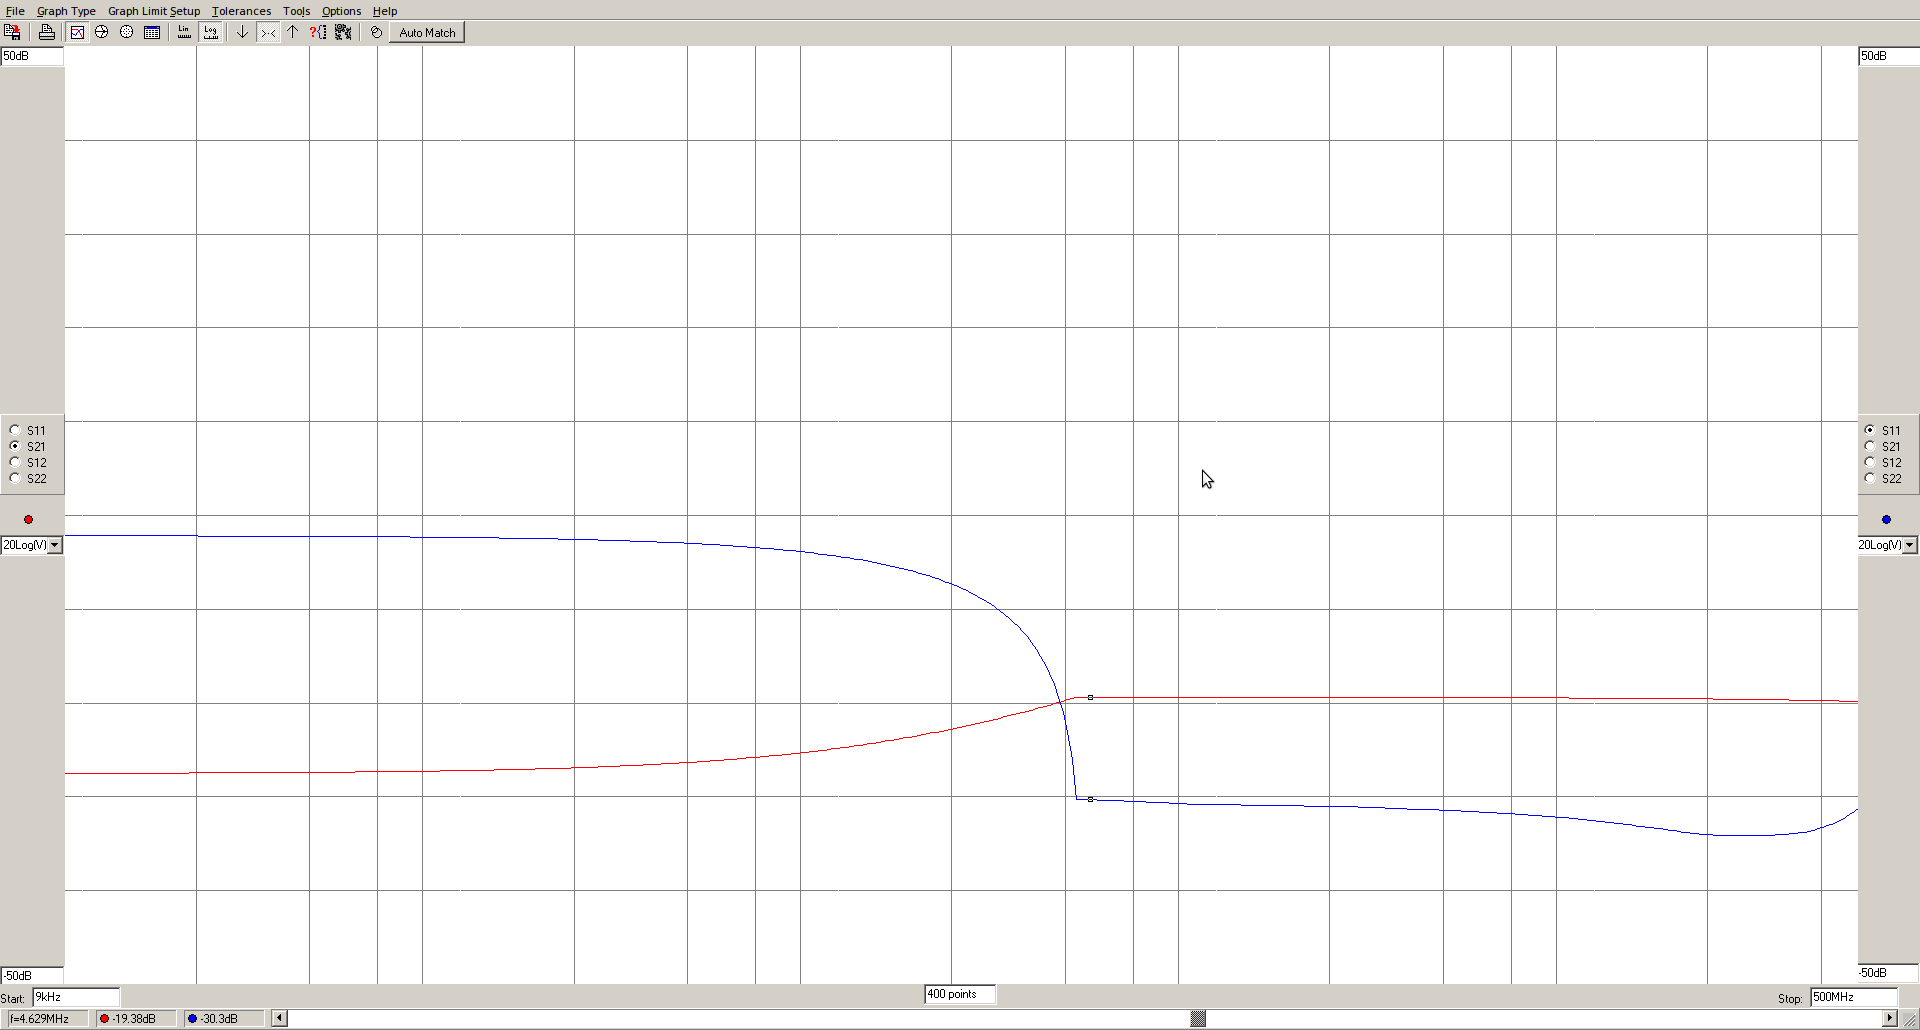
\includegraphics[scale = 0.25]{pic/cdic.png}\\\end{center}
Sur ce graphique on s'aperçoit que l'orsque le signal est addapté (-30dB) au alentour de 4MHz.
La transmission se stabilise à -20dB. Ainsi on s'apperçoit que le signal couplé n'est qu'une petit
portion du signal d'entrée.
\section{Isolation}
\subsection{Cablage}
\begin{center}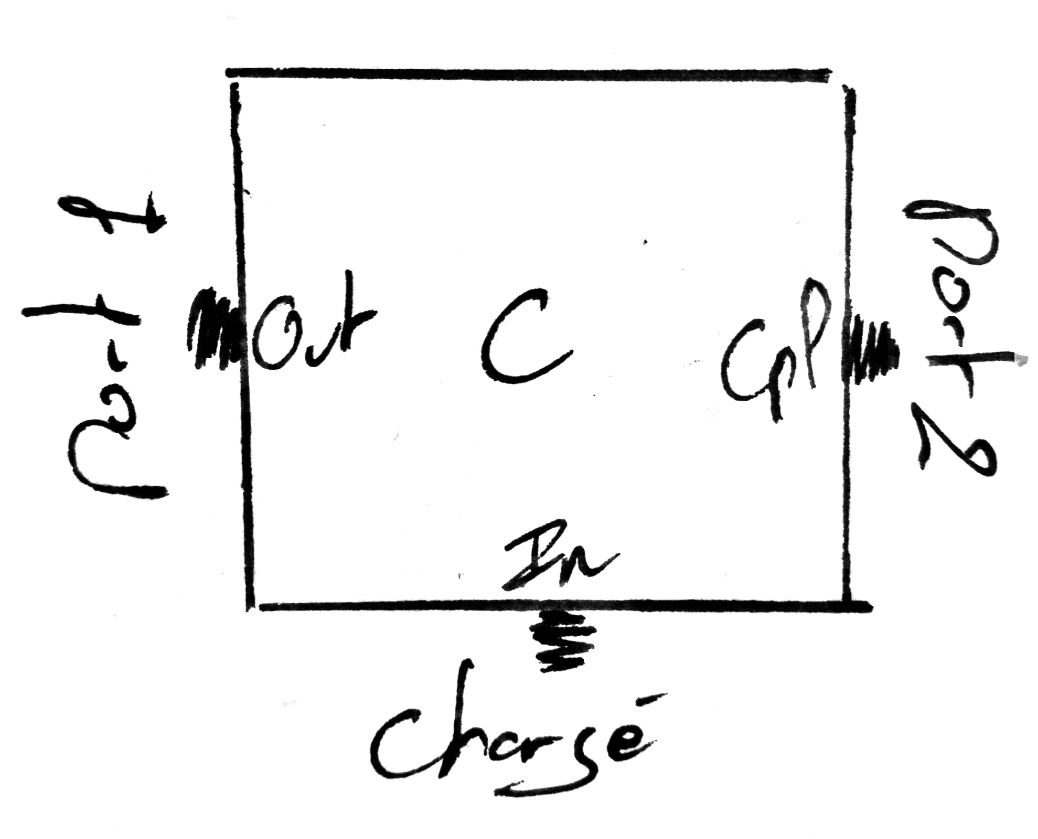
\includegraphics[scale = 0.17]{pic/CDOP.png}\\ \end{center}
De même que précédement tout port vide sera chargé.
\newpage
\subsection{Mesures}
\begin{center}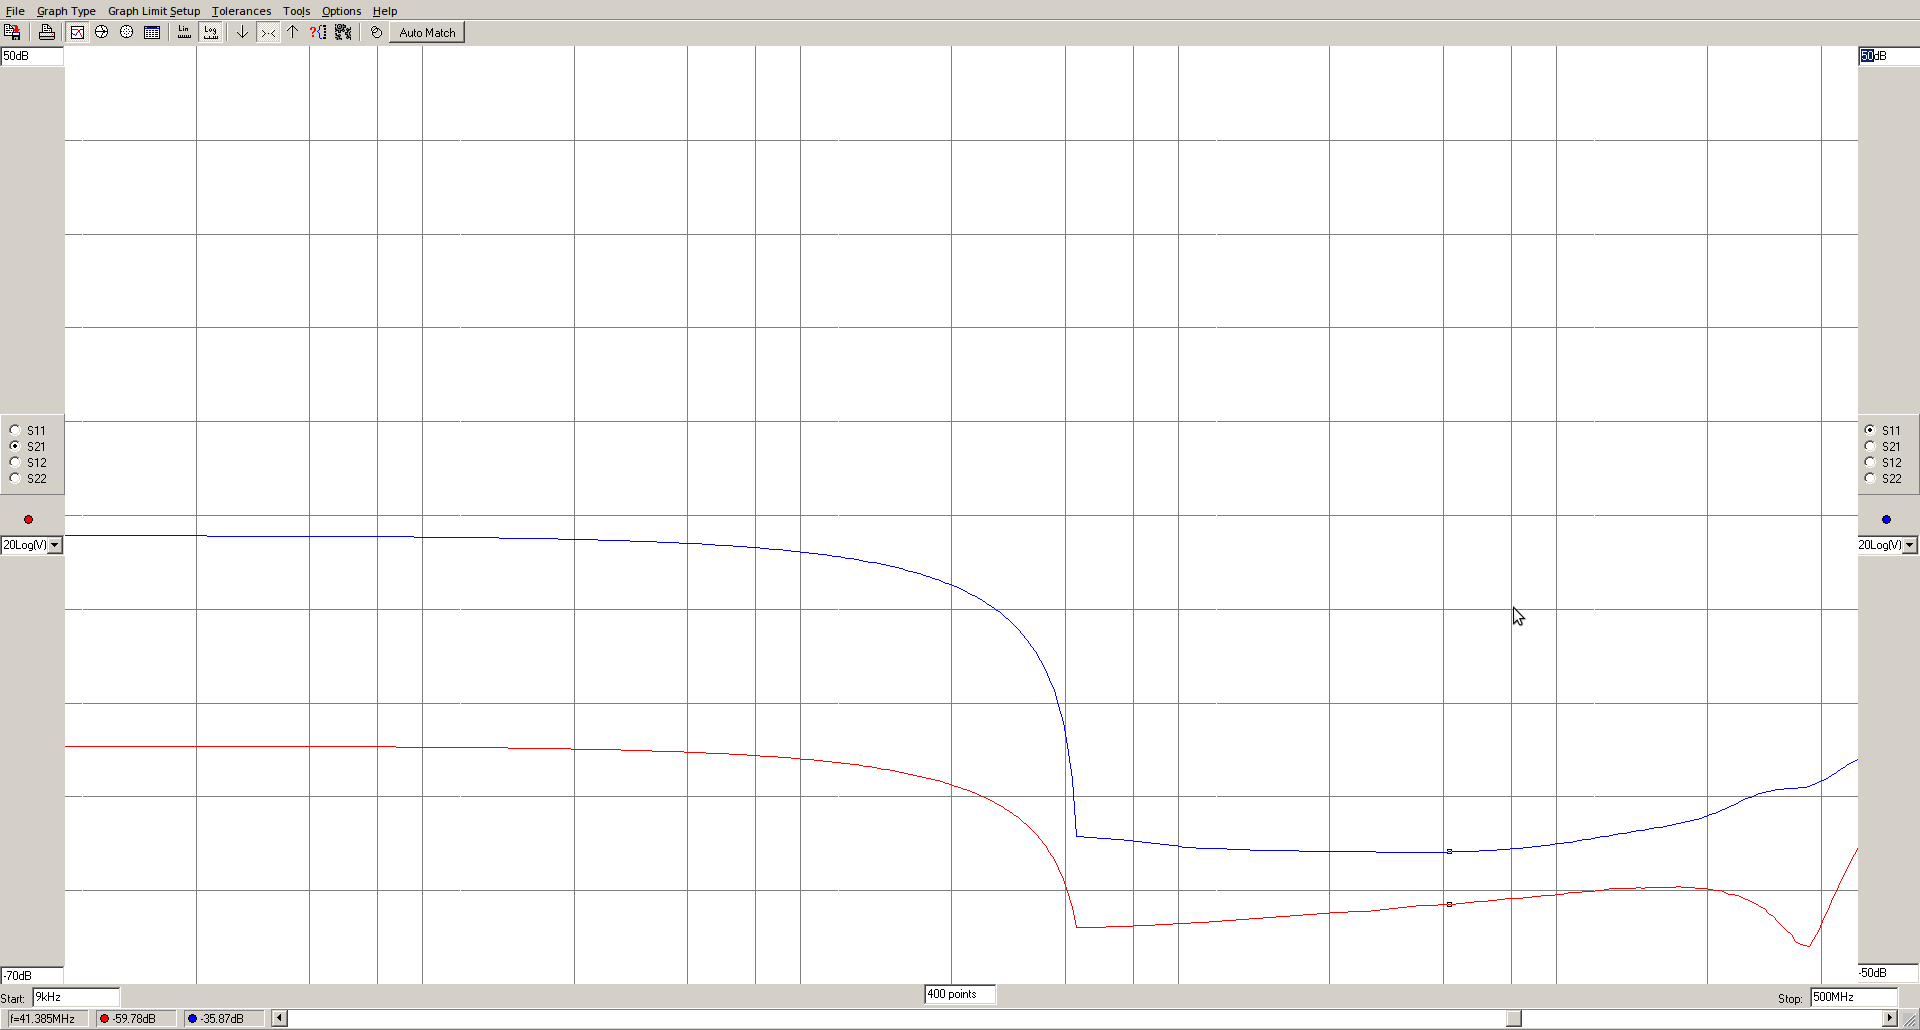
\includegraphics[scale = 0.25]{pic/cdop.png} \\\end{center}
Lorsque le système est adapté (courbe bleu a -30dB). On obtient un signal de transmission entre 
de -60dB entre la sortie et le Cpl (voir schèma). Cette transmission (courbe rouge) se trouve 
toujours en dessous de l'adaptation et influe au même moment. 
\chapter{Conclusion}
\addcontentsline{toc}{chapter}{Conclusion}
Lors de ce TP nous avons appris à nous servir de l'analyseur de réseaux. Grâce à cette appareil
nous avons pû étudier différents filtres, et déterminer leurs types (tchebychev ou butterworth). 
Puisuqe en effet de part la lecture des paraèmtres S, il est plus facil d'étudier en profondeur les 
caractéristique des objets étudier.
Nous avons ensuite étudier un diviseur de puissance et un coupleur directif. Afin de déterminer leurs
caractéristique.
A noté que tout ces composants sont passsif on retrouve donc les même signaux sur S12 et S21.
\end{document}